\documentclass[twoside]{book}

% Packages required by doxygen
\usepackage{fixltx2e}
\usepackage{calc}
\usepackage{doxygen}
\usepackage[export]{adjustbox} % also loads graphicx
\usepackage{graphicx}
\usepackage[utf8]{inputenc}
\usepackage{makeidx}
\usepackage{multicol}
\usepackage{multirow}
\PassOptionsToPackage{warn}{textcomp}
\usepackage{textcomp}
\usepackage[nointegrals]{wasysym}
\usepackage[table]{xcolor}

% Font selection
\usepackage[T1]{fontenc}
\usepackage[scaled=.90]{helvet}
\usepackage{courier}
\usepackage{amssymb}
\usepackage{sectsty}
\renewcommand{\familydefault}{\sfdefault}
\allsectionsfont{%
  \fontseries{bc}\selectfont%
  \color{darkgray}%
}
\renewcommand{\DoxyLabelFont}{%
  \fontseries{bc}\selectfont%
  \color{darkgray}%
}
\newcommand{\+}{\discretionary{\mbox{\scriptsize$\hookleftarrow$}}{}{}}

% Page & text layout
\usepackage{geometry}
\geometry{%
  a4paper,%
  top=2.5cm,%
  bottom=2.5cm,%
  left=2.5cm,%
  right=2.5cm%
}
\tolerance=750
\hfuzz=15pt
\hbadness=750
\setlength{\emergencystretch}{15pt}
\setlength{\parindent}{0cm}
\setlength{\parskip}{3ex plus 2ex minus 2ex}
\makeatletter
\renewcommand{\paragraph}{%
  \@startsection{paragraph}{4}{0ex}{-1.0ex}{1.0ex}{%
    \normalfont\normalsize\bfseries\SS@parafont%
  }%
}
\renewcommand{\subparagraph}{%
  \@startsection{subparagraph}{5}{0ex}{-1.0ex}{1.0ex}{%
    \normalfont\normalsize\bfseries\SS@subparafont%
  }%
}
\makeatother

% Headers & footers
\usepackage{fancyhdr}
\pagestyle{fancyplain}
\fancyhead[LE]{\fancyplain{}{\bfseries\thepage}}
\fancyhead[CE]{\fancyplain{}{}}
\fancyhead[RE]{\fancyplain{}{\bfseries\leftmark}}
\fancyhead[LO]{\fancyplain{}{\bfseries\rightmark}}
\fancyhead[CO]{\fancyplain{}{}}
\fancyhead[RO]{\fancyplain{}{\bfseries\thepage}}
\fancyfoot[LE]{\fancyplain{}{}}
\fancyfoot[CE]{\fancyplain{}{}}
\fancyfoot[RE]{\fancyplain{}{\bfseries\scriptsize Generated by Doxygen }}
\fancyfoot[LO]{\fancyplain{}{\bfseries\scriptsize Generated by Doxygen }}
\fancyfoot[CO]{\fancyplain{}{}}
\fancyfoot[RO]{\fancyplain{}{}}
\renewcommand{\footrulewidth}{0.4pt}
\renewcommand{\chaptermark}[1]{%
  \markboth{#1}{}%
}
\renewcommand{\sectionmark}[1]{%
  \markright{\thesection\ #1}%
}

% Indices & bibliography
\usepackage{natbib}
\usepackage[titles]{tocloft}
\setcounter{tocdepth}{3}
\setcounter{secnumdepth}{5}
\makeindex

% Hyperlinks (required, but should be loaded last)
\usepackage{ifpdf}
\ifpdf
  \usepackage[pdftex,pagebackref=true]{hyperref}
\else
  \usepackage[ps2pdf,pagebackref=true]{hyperref}
\fi
\hypersetup{%
  colorlinks=true,%
  linkcolor=blue,%
  citecolor=blue,%
  unicode%
}

% Custom commands
\newcommand{\clearemptydoublepage}{%
  \newpage{\pagestyle{empty}\cleardoublepage}%
}

\usepackage{caption}
\captionsetup{labelsep=space,justification=centering,font={bf},singlelinecheck=off,skip=4pt,position=top}

%===== C O N T E N T S =====

\begin{document}

% Titlepage & ToC
\hypersetup{pageanchor=false,
             bookmarksnumbered=true,
             pdfencoding=unicode
            }
\pagenumbering{alph}
\begin{titlepage}
\vspace*{7cm}
\begin{center}%
{\Large shrub }\\
\vspace*{1cm}
{\large Generated by Doxygen 1.8.13}\\
\end{center}
\end{titlepage}
\clearemptydoublepage
\pagenumbering{roman}
\tableofcontents
\clearemptydoublepage
\pagenumbering{arabic}
\hypersetup{pageanchor=true}

%--- Begin generated contents ---
\chapter{R\+E\+A\+D\+ME}
\label{md__r_e_a_d_m_e}
\Hypertarget{md__r_e_a_d_m_e}
This R\+E\+A\+D\+ME would normally document whatever steps are necessary to get your application up and running.

\subsubsection*{What is this repository for?}


\begin{DoxyItemize}
\item This is the repository for the code for Shrub.
\item .01a
\end{DoxyItemize}

\subsubsection*{How do I get set up?}


\begin{DoxyItemize}
\item Summary of set up
\item Configuration
\item Dependencies
\item Database configuration
\item How to run tests
\item Deployment instructions
\end{DoxyItemize}

\subsubsection*{Contribution guidelines}


\begin{DoxyItemize}
\item Writing tests
\item Code review
\item Other guidelines
\end{DoxyItemize}

\subsubsection*{Who do I talk to?}


\begin{DoxyItemize}
\item Repo owner or admin
\item Other community or team contact 
\end{DoxyItemize}
\chapter{Hierarchical Index}
\section{Class Hierarchy}
This inheritance list is sorted roughly, but not completely, alphabetically\+:\begin{DoxyCompactList}
\item \contentsline{section}{Enumerations}{\pageref{class_enumerations}}{}
\item Mono\+Behaviour\begin{DoxyCompactList}
\item \contentsline{section}{Animal}{\pageref{class_animal}}{}
\item \contentsline{section}{Button}{\pageref{class_button}}{}
\item \contentsline{section}{Camera\+Manager}{\pageref{class_camera_manager}}{}
\item \contentsline{section}{Cinematic\+Camera}{\pageref{class_cinematic_camera}}{}
\item \contentsline{section}{Controller\+Input}{\pageref{class_controller_input}}{}
\item \contentsline{section}{Entity}{\pageref{class_entity}}{}
\item \contentsline{section}{Entity\+Builder}{\pageref{class_entity_builder}}{}
\item \contentsline{section}{Entity\+Dictionary}{\pageref{class_entity_dictionary}}{}
\item \contentsline{section}{Entity\+Manager}{\pageref{class_entity_manager}}{}
\item \contentsline{section}{First\+Person\+Camera}{\pageref{class_first_person_camera}}{}
\item \contentsline{section}{Forest}{\pageref{class_forest}}{}
\item \contentsline{section}{Graphic}{\pageref{class_graphic}}{}
\item \contentsline{section}{House}{\pageref{class_house}}{}
\item \contentsline{section}{Human}{\pageref{class_human}}{}
\item \contentsline{section}{Input\+Manager}{\pageref{class_input_manager}}{}
\item \contentsline{section}{Isometric\+Camera}{\pageref{class_isometric_camera}}{}
\item \contentsline{section}{Landscape}{\pageref{class_landscape}}{}
\item \contentsline{section}{Landscape\+Builder}{\pageref{class_landscape_builder}}{}
\item \contentsline{section}{Landscape\+Dictionary}{\pageref{class_landscape_dictionary}}{}
\item \contentsline{section}{Landscape\+Manager}{\pageref{class_landscape_manager}}{}
\item \contentsline{section}{Mountain}{\pageref{class_mountain}}{}
\item \contentsline{section}{Mouse\+Input}{\pageref{class_mouse_input}}{}
\item \contentsline{section}{Panel}{\pageref{class_panel}}{}
\item \contentsline{section}{Plain}{\pageref{class_plain}}{}
\item \contentsline{section}{River}{\pageref{class_river}}{}
\item \contentsline{section}{Scene\+Manager}{\pageref{class_scene_manager}}{}
\item \contentsline{section}{Third\+Person\+Camera}{\pageref{class_third_person_camera}}{}
\item \contentsline{section}{Touch\+Input}{\pageref{class_touch_input}}{}
\item \contentsline{section}{U\+I\+Manager}{\pageref{class_u_i_manager}}{}
\end{DoxyCompactList}
\end{DoxyCompactList}

\chapter{Class Index}
\section{Class List}
Here are the classes, structs, unions and interfaces with brief descriptions\+:\begin{DoxyCompactList}
\item\contentsline{section}{\hyperlink{class_animal}{Animal} }{\pageref{class_animal}}{}
\item\contentsline{section}{\hyperlink{class_button}{Button} }{\pageref{class_button}}{}
\item\contentsline{section}{\hyperlink{class_camera_manager}{Camera\+Manager} }{\pageref{class_camera_manager}}{}
\item\contentsline{section}{\hyperlink{class_cinematic_camera}{Cinematic\+Camera} }{\pageref{class_cinematic_camera}}{}
\item\contentsline{section}{\hyperlink{class_controller_input}{Controller\+Input} }{\pageref{class_controller_input}}{}
\item\contentsline{section}{\hyperlink{class_entity}{Entity} }{\pageref{class_entity}}{}
\item\contentsline{section}{\hyperlink{class_entity_builder}{Entity\+Builder} }{\pageref{class_entity_builder}}{}
\item\contentsline{section}{\hyperlink{class_entity_dictionary}{Entity\+Dictionary} }{\pageref{class_entity_dictionary}}{}
\item\contentsline{section}{\hyperlink{class_entity_manager}{Entity\+Manager} }{\pageref{class_entity_manager}}{}
\item\contentsline{section}{\hyperlink{class_enumerations}{Enumerations} }{\pageref{class_enumerations}}{}
\item\contentsline{section}{\hyperlink{class_first_person_camera}{First\+Person\+Camera} }{\pageref{class_first_person_camera}}{}
\item\contentsline{section}{\hyperlink{class_forest}{Forest} }{\pageref{class_forest}}{}
\item\contentsline{section}{\hyperlink{class_graphic}{Graphic} }{\pageref{class_graphic}}{}
\item\contentsline{section}{\hyperlink{class_house}{House} }{\pageref{class_house}}{}
\item\contentsline{section}{\hyperlink{class_human}{Human} }{\pageref{class_human}}{}
\item\contentsline{section}{\hyperlink{class_input_manager}{Input\+Manager} }{\pageref{class_input_manager}}{}
\item\contentsline{section}{\hyperlink{class_isometric_camera}{Isometric\+Camera} }{\pageref{class_isometric_camera}}{}
\item\contentsline{section}{\hyperlink{class_landscape}{Landscape} }{\pageref{class_landscape}}{}
\item\contentsline{section}{\hyperlink{class_landscape_builder}{Landscape\+Builder} }{\pageref{class_landscape_builder}}{}
\item\contentsline{section}{\hyperlink{class_landscape_dictionary}{Landscape\+Dictionary} }{\pageref{class_landscape_dictionary}}{}
\item\contentsline{section}{\hyperlink{class_landscape_manager}{Landscape\+Manager} }{\pageref{class_landscape_manager}}{}
\item\contentsline{section}{\hyperlink{class_mountain}{Mountain} }{\pageref{class_mountain}}{}
\item\contentsline{section}{\hyperlink{class_mouse_input}{Mouse\+Input} }{\pageref{class_mouse_input}}{}
\item\contentsline{section}{\hyperlink{class_panel}{Panel} }{\pageref{class_panel}}{}
\item\contentsline{section}{\hyperlink{class_plain}{Plain} }{\pageref{class_plain}}{}
\item\contentsline{section}{\hyperlink{class_river}{River} }{\pageref{class_river}}{}
\item\contentsline{section}{\hyperlink{class_scene_manager}{Scene\+Manager} }{\pageref{class_scene_manager}}{}
\item\contentsline{section}{\hyperlink{class_third_person_camera}{Third\+Person\+Camera} }{\pageref{class_third_person_camera}}{}
\item\contentsline{section}{\hyperlink{class_touch_input}{Touch\+Input} }{\pageref{class_touch_input}}{}
\item\contentsline{section}{\hyperlink{class_u_i_manager}{U\+I\+Manager} }{\pageref{class_u_i_manager}}{}
\end{DoxyCompactList}

\chapter{File Index}
\section{File List}
Here is a list of all files with brief descriptions\+:\begin{DoxyCompactList}
\item\contentsline{section}{Assets/\hyperlink{_animal_8cs}{Animal.\+cs} }{\pageref{_animal_8cs}}{}
\item\contentsline{section}{Assets/\hyperlink{_button_8cs}{Button.\+cs} }{\pageref{_button_8cs}}{}
\item\contentsline{section}{Assets/\hyperlink{_camera_manager_8cs}{Camera\+Manager.\+cs} }{\pageref{_camera_manager_8cs}}{}
\item\contentsline{section}{Assets/\hyperlink{_cinematic_camera_8cs}{Cinematic\+Camera.\+cs} }{\pageref{_cinematic_camera_8cs}}{}
\item\contentsline{section}{Assets/\hyperlink{_controller_input_8cs}{Controller\+Input.\+cs} }{\pageref{_controller_input_8cs}}{}
\item\contentsline{section}{Assets/\hyperlink{_entity_8cs}{Entity.\+cs} }{\pageref{_entity_8cs}}{}
\item\contentsline{section}{Assets/\hyperlink{_entity_builder_8cs}{Entity\+Builder.\+cs} }{\pageref{_entity_builder_8cs}}{}
\item\contentsline{section}{Assets/\hyperlink{_entity_dictionary_8cs}{Entity\+Dictionary.\+cs} }{\pageref{_entity_dictionary_8cs}}{}
\item\contentsline{section}{Assets/\hyperlink{_entity_manager_8cs}{Entity\+Manager.\+cs} }{\pageref{_entity_manager_8cs}}{}
\item\contentsline{section}{Assets/\hyperlink{_enumerations_8cs}{Enumerations.\+cs} }{\pageref{_enumerations_8cs}}{}
\item\contentsline{section}{Assets/\hyperlink{_first_person_camera_8cs}{First\+Person\+Camera.\+cs} }{\pageref{_first_person_camera_8cs}}{}
\item\contentsline{section}{Assets/\hyperlink{_forest_8cs}{Forest.\+cs} }{\pageref{_forest_8cs}}{}
\item\contentsline{section}{Assets/\hyperlink{_graphic_8cs}{Graphic.\+cs} }{\pageref{_graphic_8cs}}{}
\item\contentsline{section}{Assets/\hyperlink{_house_8cs}{House.\+cs} }{\pageref{_house_8cs}}{}
\item\contentsline{section}{Assets/\hyperlink{_human_8cs}{Human.\+cs} }{\pageref{_human_8cs}}{}
\item\contentsline{section}{Assets/\hyperlink{_input_manager_8cs}{Input\+Manager.\+cs} }{\pageref{_input_manager_8cs}}{}
\item\contentsline{section}{Assets/\hyperlink{_isometric_camera_8cs}{Isometric\+Camera.\+cs} }{\pageref{_isometric_camera_8cs}}{}
\item\contentsline{section}{Assets/\hyperlink{_landscape_8cs}{Landscape.\+cs} }{\pageref{_landscape_8cs}}{}
\item\contentsline{section}{Assets/\hyperlink{_landscape_builder_8cs}{Landscape\+Builder.\+cs} }{\pageref{_landscape_builder_8cs}}{}
\item\contentsline{section}{Assets/\hyperlink{_landscape_dictionary_8cs}{Landscape\+Dictionary.\+cs} }{\pageref{_landscape_dictionary_8cs}}{}
\item\contentsline{section}{Assets/\hyperlink{_landscape_manager_8cs}{Landscape\+Manager.\+cs} }{\pageref{_landscape_manager_8cs}}{}
\item\contentsline{section}{Assets/\hyperlink{_mountain_8cs}{Mountain.\+cs} }{\pageref{_mountain_8cs}}{}
\item\contentsline{section}{Assets/\hyperlink{_mouse_input_8cs}{Mouse\+Input.\+cs} }{\pageref{_mouse_input_8cs}}{}
\item\contentsline{section}{Assets/\hyperlink{_panel_8cs}{Panel.\+cs} }{\pageref{_panel_8cs}}{}
\item\contentsline{section}{Assets/\hyperlink{_plain_8cs}{Plain.\+cs} }{\pageref{_plain_8cs}}{}
\item\contentsline{section}{Assets/\hyperlink{_river_8cs}{River.\+cs} }{\pageref{_river_8cs}}{}
\item\contentsline{section}{Assets/\hyperlink{_scene_manager_8cs}{Scene\+Manager.\+cs} }{\pageref{_scene_manager_8cs}}{}
\item\contentsline{section}{Assets/\hyperlink{_third_person_camera_8cs}{Third\+Person\+Camera.\+cs} }{\pageref{_third_person_camera_8cs}}{}
\item\contentsline{section}{Assets/\hyperlink{_touch_input_8cs}{Touch\+Input.\+cs} }{\pageref{_touch_input_8cs}}{}
\item\contentsline{section}{Assets/\hyperlink{_u_i_manager_8cs}{U\+I\+Manager.\+cs} }{\pageref{_u_i_manager_8cs}}{}
\end{DoxyCompactList}

\chapter{Class Documentation}
\hypertarget{class_animal}{}\section{Animal Class Reference}
\label{class_animal}\index{Animal@{Animal}}
Inheritance diagram for Animal\+:\begin{figure}[H]
\begin{center}
\leavevmode
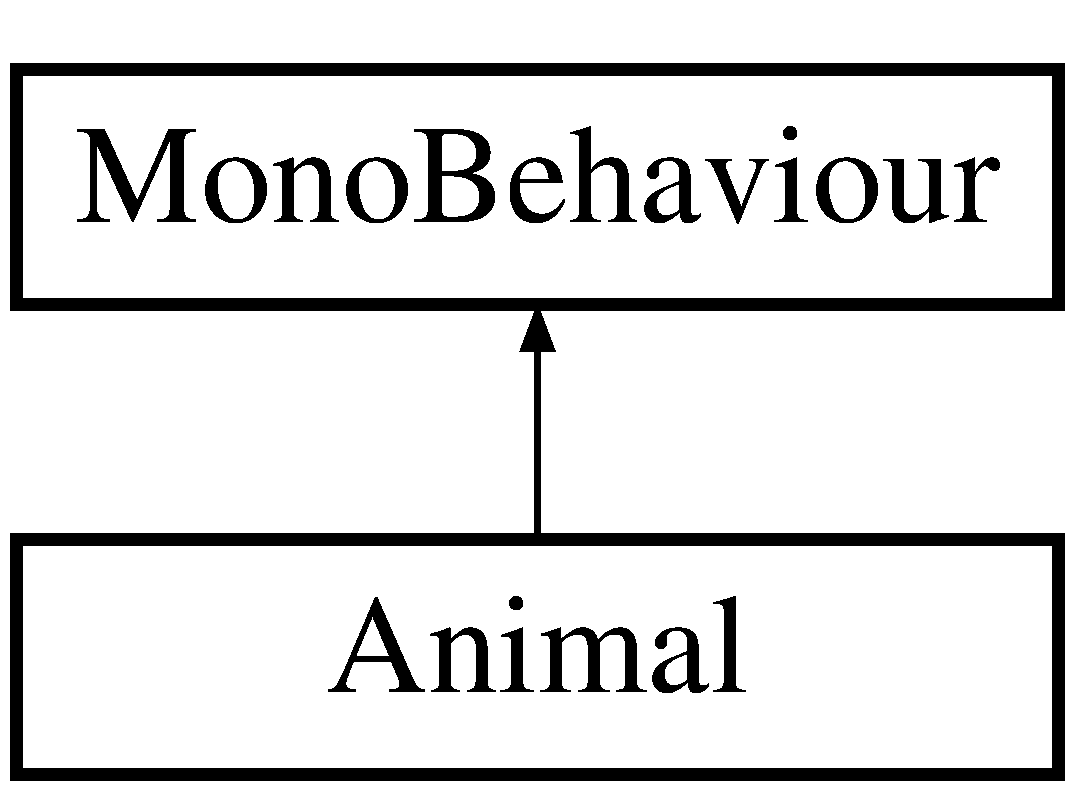
\includegraphics[height=2.000000cm]{class_animal}
\end{center}
\end{figure}
\subsection*{Private Member Functions}
\begin{DoxyCompactItemize}
\item 
void \hyperlink{class_animal_a575af2ae0415ed0fece71e6faba71979}{Start} ()
\item 
void \hyperlink{class_animal_a8efd540bef3e9d7776eedae9020ec41c}{Update} ()
\end{DoxyCompactItemize}


\subsection{Member Function Documentation}
\mbox{\Hypertarget{class_animal_a575af2ae0415ed0fece71e6faba71979}\label{class_animal_a575af2ae0415ed0fece71e6faba71979}} 
\index{Animal@{Animal}!Start@{Start}}
\index{Start@{Start}!Animal@{Animal}}
\subsubsection{\texorpdfstring{Start()}{Start()}}
{\footnotesize\ttfamily void Animal.\+Start (\begin{DoxyParamCaption}{ }\end{DoxyParamCaption})\hspace{0.3cm}{\ttfamily [private]}}

\mbox{\Hypertarget{class_animal_a8efd540bef3e9d7776eedae9020ec41c}\label{class_animal_a8efd540bef3e9d7776eedae9020ec41c}} 
\index{Animal@{Animal}!Update@{Update}}
\index{Update@{Update}!Animal@{Animal}}
\subsubsection{\texorpdfstring{Update()}{Update()}}
{\footnotesize\ttfamily void Animal.\+Update (\begin{DoxyParamCaption}{ }\end{DoxyParamCaption})\hspace{0.3cm}{\ttfamily [private]}}



The documentation for this class was generated from the following file\+:\begin{DoxyCompactItemize}
\item 
Assets/\hyperlink{_animal_8cs}{Animal.\+cs}\end{DoxyCompactItemize}

\hypertarget{class_button}{}\section{Button Class Reference}
\label{class_button}\index{Button@{Button}}
Inheritance diagram for Button\+:\begin{figure}[H]
\begin{center}
\leavevmode
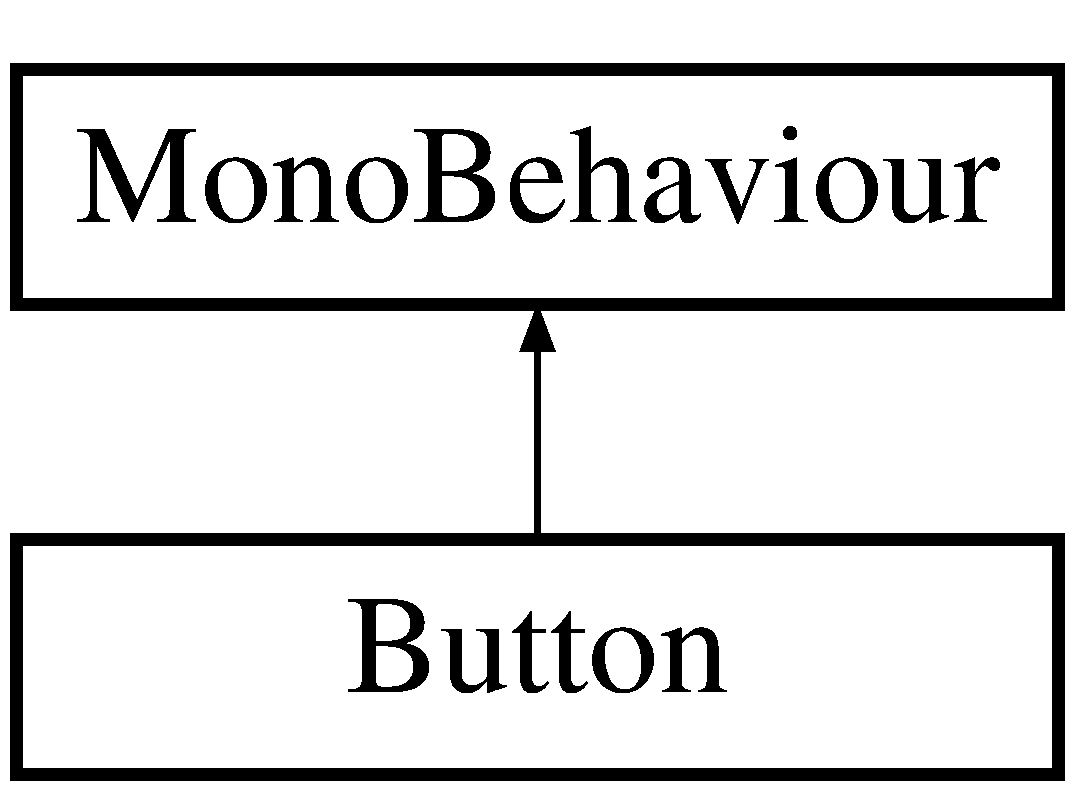
\includegraphics[height=2.000000cm]{class_button}
\end{center}
\end{figure}
\subsection*{Private Member Functions}
\begin{DoxyCompactItemize}
\item 
void \hyperlink{class_button_a1ca1f623a8d5f7e9453eee7698e216ec}{Start} ()
\item 
void \hyperlink{class_button_abde2585e345c77634cc81b2f46c24936}{Update} ()
\end{DoxyCompactItemize}


\subsection{Member Function Documentation}
\mbox{\Hypertarget{class_button_a1ca1f623a8d5f7e9453eee7698e216ec}\label{class_button_a1ca1f623a8d5f7e9453eee7698e216ec}} 
\index{Button@{Button}!Start@{Start}}
\index{Start@{Start}!Button@{Button}}
\subsubsection{\texorpdfstring{Start()}{Start()}}
{\footnotesize\ttfamily void Button.\+Start (\begin{DoxyParamCaption}{ }\end{DoxyParamCaption})\hspace{0.3cm}{\ttfamily [private]}}

\mbox{\Hypertarget{class_button_abde2585e345c77634cc81b2f46c24936}\label{class_button_abde2585e345c77634cc81b2f46c24936}} 
\index{Button@{Button}!Update@{Update}}
\index{Update@{Update}!Button@{Button}}
\subsubsection{\texorpdfstring{Update()}{Update()}}
{\footnotesize\ttfamily void Button.\+Update (\begin{DoxyParamCaption}{ }\end{DoxyParamCaption})\hspace{0.3cm}{\ttfamily [private]}}



The documentation for this class was generated from the following file\+:\begin{DoxyCompactItemize}
\item 
Assets/\hyperlink{_button_8cs}{Button.\+cs}\end{DoxyCompactItemize}

\hypertarget{class_camera_manager}{}\section{Camera\+Manager Class Reference}
\label{class_camera_manager}\index{Camera\+Manager@{Camera\+Manager}}
Inheritance diagram for Camera\+Manager\+:\begin{figure}[H]
\begin{center}
\leavevmode
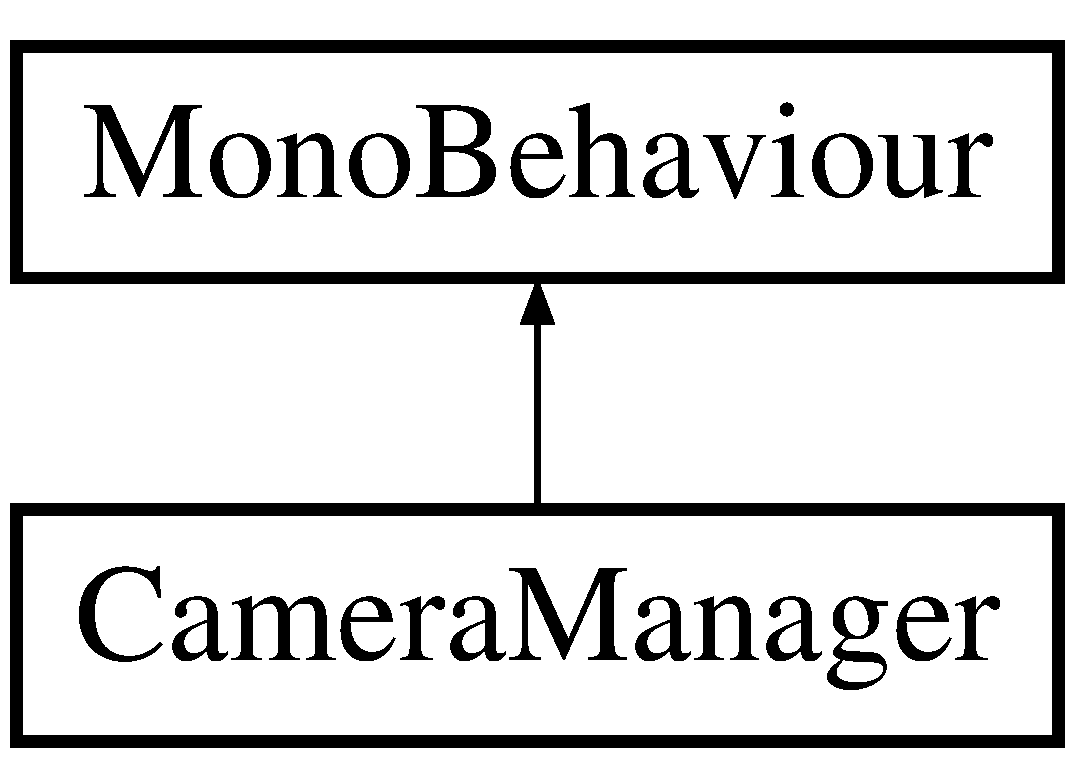
\includegraphics[height=2.000000cm]{class_camera_manager}
\end{center}
\end{figure}
\subsection*{Private Member Functions}
\begin{DoxyCompactItemize}
\item 
void \hyperlink{class_camera_manager_a5010f55d95e2b09bf041387388a38ec1}{Start} ()
\item 
void \hyperlink{class_camera_manager_a10cfc1f1e06a1ebd569c60b48261a692}{Update} ()
\end{DoxyCompactItemize}


\subsection{Member Function Documentation}
\mbox{\Hypertarget{class_camera_manager_a5010f55d95e2b09bf041387388a38ec1}\label{class_camera_manager_a5010f55d95e2b09bf041387388a38ec1}} 
\index{Camera\+Manager@{Camera\+Manager}!Start@{Start}}
\index{Start@{Start}!Camera\+Manager@{Camera\+Manager}}
\subsubsection{\texorpdfstring{Start()}{Start()}}
{\footnotesize\ttfamily void Camera\+Manager.\+Start (\begin{DoxyParamCaption}{ }\end{DoxyParamCaption})\hspace{0.3cm}{\ttfamily [private]}}

\mbox{\Hypertarget{class_camera_manager_a10cfc1f1e06a1ebd569c60b48261a692}\label{class_camera_manager_a10cfc1f1e06a1ebd569c60b48261a692}} 
\index{Camera\+Manager@{Camera\+Manager}!Update@{Update}}
\index{Update@{Update}!Camera\+Manager@{Camera\+Manager}}
\subsubsection{\texorpdfstring{Update()}{Update()}}
{\footnotesize\ttfamily void Camera\+Manager.\+Update (\begin{DoxyParamCaption}{ }\end{DoxyParamCaption})\hspace{0.3cm}{\ttfamily [private]}}



The documentation for this class was generated from the following file\+:\begin{DoxyCompactItemize}
\item 
Assets/\hyperlink{_camera_manager_8cs}{Camera\+Manager.\+cs}\end{DoxyCompactItemize}

\hypertarget{class_cinematic_camera}{}\section{Cinematic\+Camera Class Reference}
\label{class_cinematic_camera}\index{Cinematic\+Camera@{Cinematic\+Camera}}
Inheritance diagram for Cinematic\+Camera\+:\begin{figure}[H]
\begin{center}
\leavevmode
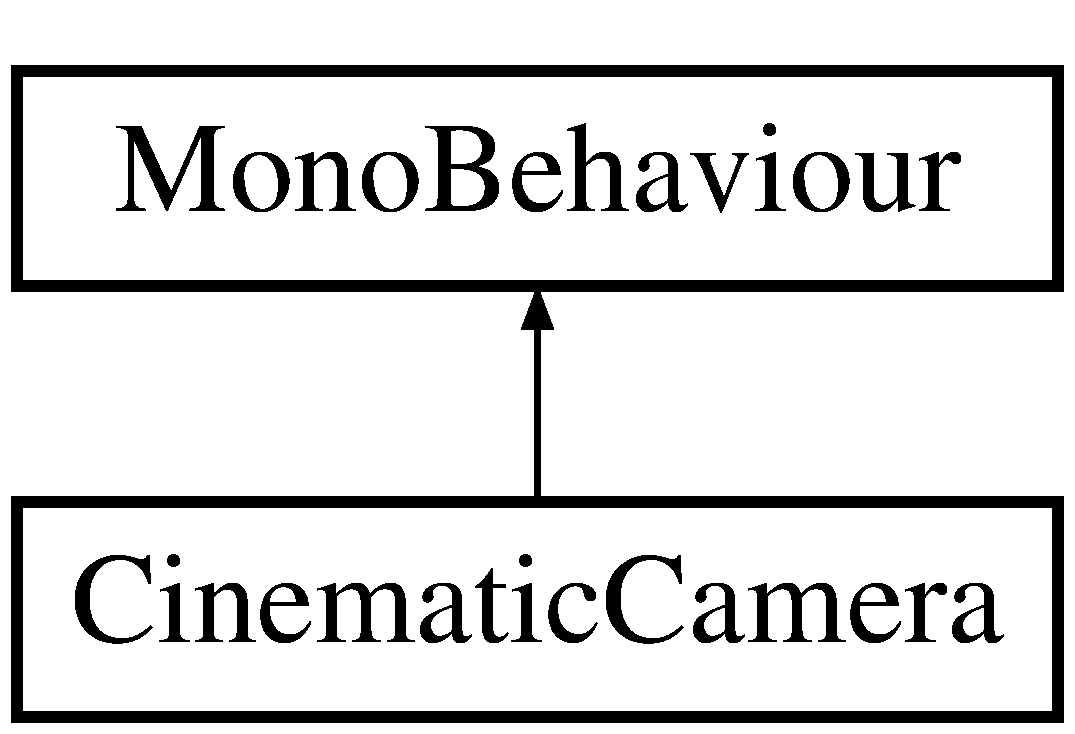
\includegraphics[height=2.000000cm]{class_cinematic_camera}
\end{center}
\end{figure}
\subsection*{Private Member Functions}
\begin{DoxyCompactItemize}
\item 
void \hyperlink{class_cinematic_camera_a7725aed0091d59f81793a0d7625a3e74}{Start} ()
\item 
void \hyperlink{class_cinematic_camera_a5716ab0ee2ce8829223cce6670cf5f2f}{Update} ()
\end{DoxyCompactItemize}


\subsection{Member Function Documentation}
\mbox{\Hypertarget{class_cinematic_camera_a7725aed0091d59f81793a0d7625a3e74}\label{class_cinematic_camera_a7725aed0091d59f81793a0d7625a3e74}} 
\index{Cinematic\+Camera@{Cinematic\+Camera}!Start@{Start}}
\index{Start@{Start}!Cinematic\+Camera@{Cinematic\+Camera}}
\subsubsection{\texorpdfstring{Start()}{Start()}}
{\footnotesize\ttfamily void Cinematic\+Camera.\+Start (\begin{DoxyParamCaption}{ }\end{DoxyParamCaption})\hspace{0.3cm}{\ttfamily [private]}}

\mbox{\Hypertarget{class_cinematic_camera_a5716ab0ee2ce8829223cce6670cf5f2f}\label{class_cinematic_camera_a5716ab0ee2ce8829223cce6670cf5f2f}} 
\index{Cinematic\+Camera@{Cinematic\+Camera}!Update@{Update}}
\index{Update@{Update}!Cinematic\+Camera@{Cinematic\+Camera}}
\subsubsection{\texorpdfstring{Update()}{Update()}}
{\footnotesize\ttfamily void Cinematic\+Camera.\+Update (\begin{DoxyParamCaption}{ }\end{DoxyParamCaption})\hspace{0.3cm}{\ttfamily [private]}}



The documentation for this class was generated from the following file\+:\begin{DoxyCompactItemize}
\item 
Assets/\hyperlink{_cinematic_camera_8cs}{Cinematic\+Camera.\+cs}\end{DoxyCompactItemize}

\hypertarget{class_controller_input}{}\section{Controller\+Input Class Reference}
\label{class_controller_input}\index{Controller\+Input@{Controller\+Input}}
Inheritance diagram for Controller\+Input\+:\begin{figure}[H]
\begin{center}
\leavevmode
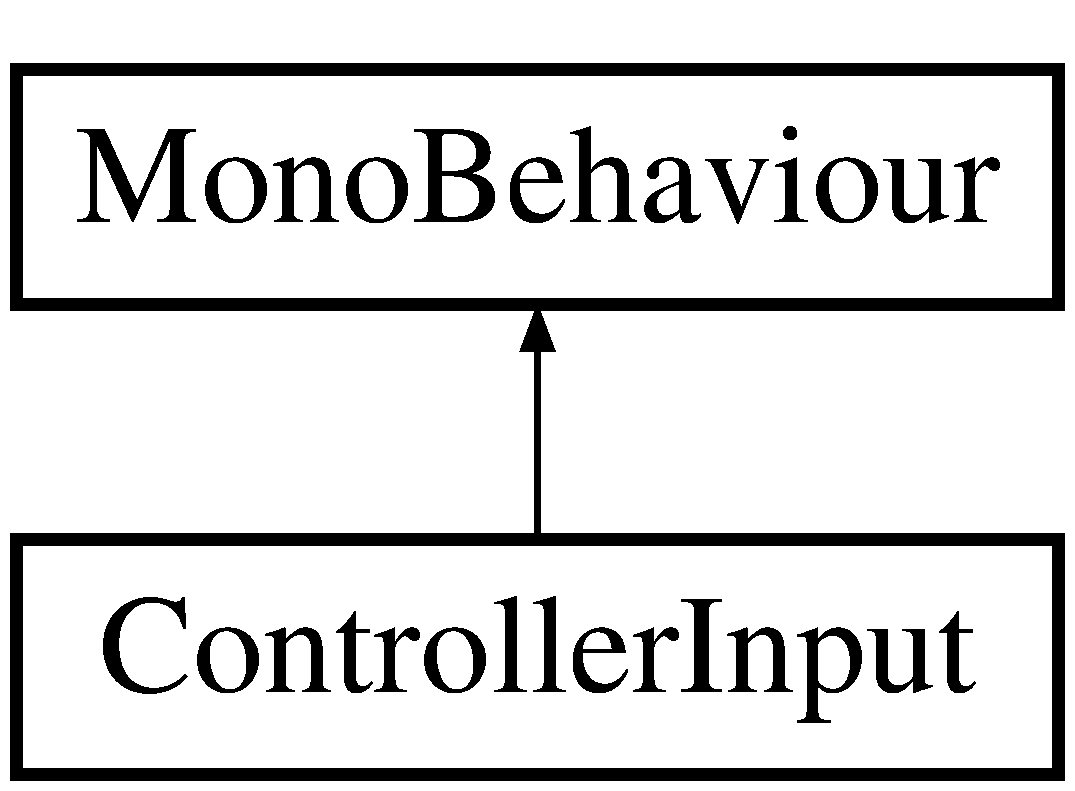
\includegraphics[height=2.000000cm]{class_controller_input}
\end{center}
\end{figure}
\subsection*{Private Member Functions}
\begin{DoxyCompactItemize}
\item 
void \hyperlink{class_controller_input_a57631a3a94346974f8db61537186f8d4}{Start} ()
\item 
void \hyperlink{class_controller_input_a37b3daf7614d8502a772b6f9a17317ed}{Update} ()
\end{DoxyCompactItemize}


\subsection{Member Function Documentation}
\mbox{\Hypertarget{class_controller_input_a57631a3a94346974f8db61537186f8d4}\label{class_controller_input_a57631a3a94346974f8db61537186f8d4}} 
\index{Controller\+Input@{Controller\+Input}!Start@{Start}}
\index{Start@{Start}!Controller\+Input@{Controller\+Input}}
\subsubsection{\texorpdfstring{Start()}{Start()}}
{\footnotesize\ttfamily void Controller\+Input.\+Start (\begin{DoxyParamCaption}{ }\end{DoxyParamCaption})\hspace{0.3cm}{\ttfamily [private]}}

\mbox{\Hypertarget{class_controller_input_a37b3daf7614d8502a772b6f9a17317ed}\label{class_controller_input_a37b3daf7614d8502a772b6f9a17317ed}} 
\index{Controller\+Input@{Controller\+Input}!Update@{Update}}
\index{Update@{Update}!Controller\+Input@{Controller\+Input}}
\subsubsection{\texorpdfstring{Update()}{Update()}}
{\footnotesize\ttfamily void Controller\+Input.\+Update (\begin{DoxyParamCaption}{ }\end{DoxyParamCaption})\hspace{0.3cm}{\ttfamily [private]}}



The documentation for this class was generated from the following file\+:\begin{DoxyCompactItemize}
\item 
Assets/\hyperlink{_controller_input_8cs}{Controller\+Input.\+cs}\end{DoxyCompactItemize}

\hypertarget{class_entity}{}\section{Entity Class Reference}
\label{class_entity}\index{Entity@{Entity}}
Inheritance diagram for Entity\+:\begin{figure}[H]
\begin{center}
\leavevmode
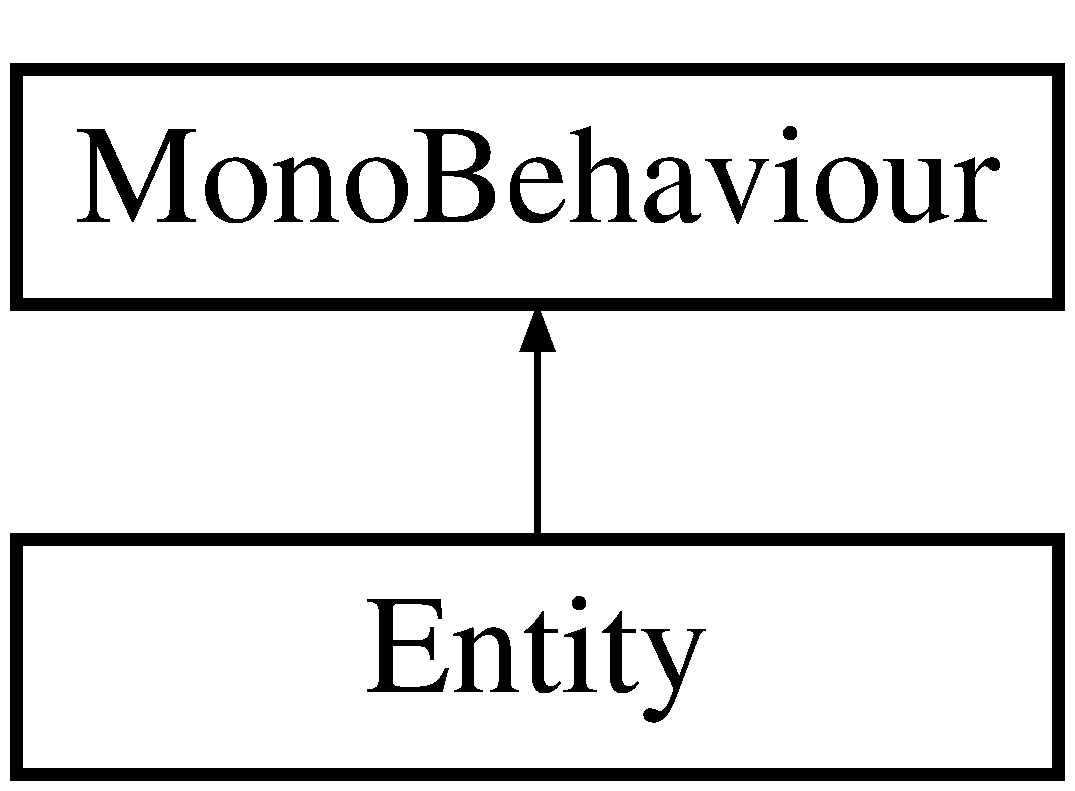
\includegraphics[height=2.000000cm]{class_entity}
\end{center}
\end{figure}
\subsection*{Private Member Functions}
\begin{DoxyCompactItemize}
\item 
void \hyperlink{class_entity_af8f28f64bf5e3c10504fda297df36e7a}{Start} ()
\item 
void \hyperlink{class_entity_affb7f61936022527f11a05baaab79b2a}{Update} ()
\end{DoxyCompactItemize}


\subsection{Member Function Documentation}
\mbox{\Hypertarget{class_entity_af8f28f64bf5e3c10504fda297df36e7a}\label{class_entity_af8f28f64bf5e3c10504fda297df36e7a}} 
\index{Entity@{Entity}!Start@{Start}}
\index{Start@{Start}!Entity@{Entity}}
\subsubsection{\texorpdfstring{Start()}{Start()}}
{\footnotesize\ttfamily void Entity.\+Start (\begin{DoxyParamCaption}{ }\end{DoxyParamCaption})\hspace{0.3cm}{\ttfamily [private]}}

\mbox{\Hypertarget{class_entity_affb7f61936022527f11a05baaab79b2a}\label{class_entity_affb7f61936022527f11a05baaab79b2a}} 
\index{Entity@{Entity}!Update@{Update}}
\index{Update@{Update}!Entity@{Entity}}
\subsubsection{\texorpdfstring{Update()}{Update()}}
{\footnotesize\ttfamily void Entity.\+Update (\begin{DoxyParamCaption}{ }\end{DoxyParamCaption})\hspace{0.3cm}{\ttfamily [private]}}



The documentation for this class was generated from the following file\+:\begin{DoxyCompactItemize}
\item 
Assets/\hyperlink{_entity_8cs}{Entity.\+cs}\end{DoxyCompactItemize}

\hypertarget{class_entity_builder}{}\section{Entity\+Builder Class Reference}
\label{class_entity_builder}\index{Entity\+Builder@{Entity\+Builder}}
Inheritance diagram for Entity\+Builder\+:\begin{figure}[H]
\begin{center}
\leavevmode
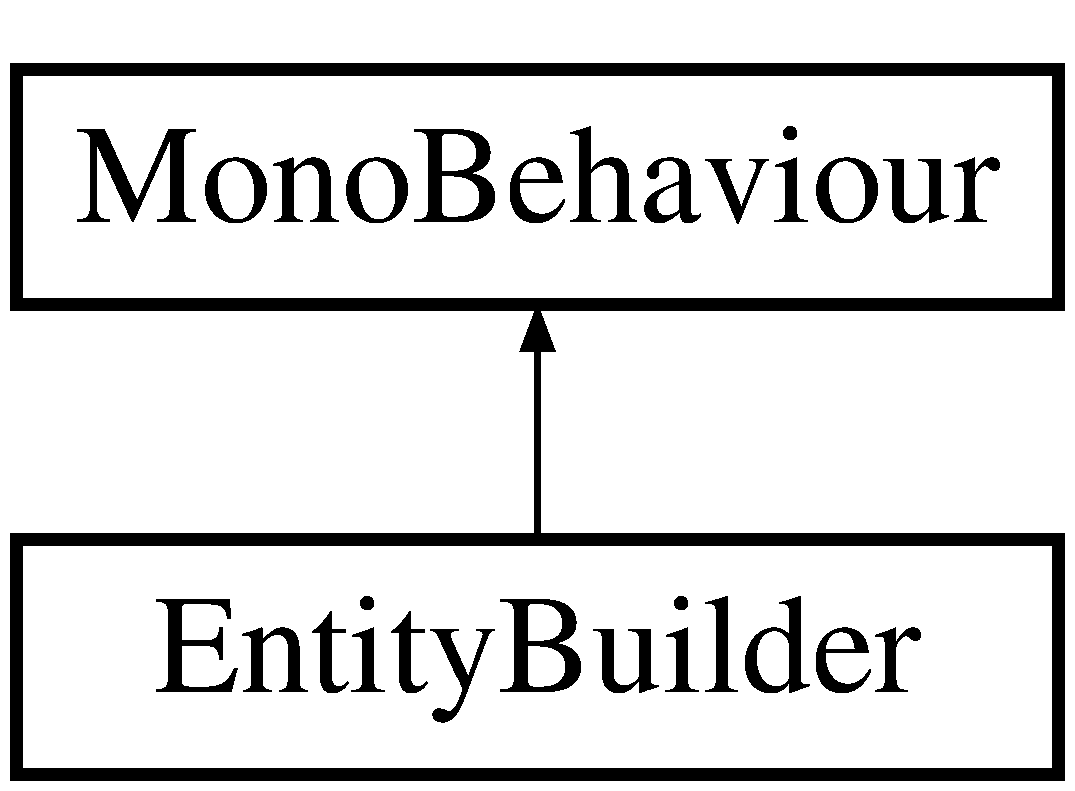
\includegraphics[height=2.000000cm]{class_entity_builder}
\end{center}
\end{figure}
\subsection*{Private Member Functions}
\begin{DoxyCompactItemize}
\item 
void \hyperlink{class_entity_builder_a2a1ce76c5e5723d2b95bab7df1adb2a5}{Start} ()
\item 
void \hyperlink{class_entity_builder_adc89d08acf62e569d3845fe95fe06611}{Update} ()
\end{DoxyCompactItemize}
\subsection*{Private Attributes}
\begin{DoxyCompactItemize}
\item 
\hyperlink{class_entity_dictionary}{Entity\+Dictionary} \hyperlink{class_entity_builder_aff80495cf34b829bdb775ef12ad3bf2e}{m\+\_\+entity\+Dictionary}
\begin{DoxyCompactList}\small\item\em The dictionary of methods by which \hyperlink{class_entity_builder}{Entity\+Builder} builds \hyperlink{class_entity}{Entity} objects. \end{DoxyCompactList}\end{DoxyCompactItemize}


\subsection{Member Function Documentation}
\mbox{\Hypertarget{class_entity_builder_a2a1ce76c5e5723d2b95bab7df1adb2a5}\label{class_entity_builder_a2a1ce76c5e5723d2b95bab7df1adb2a5}} 
\index{Entity\+Builder@{Entity\+Builder}!Start@{Start}}
\index{Start@{Start}!Entity\+Builder@{Entity\+Builder}}
\subsubsection{\texorpdfstring{Start()}{Start()}}
{\footnotesize\ttfamily void Entity\+Builder.\+Start (\begin{DoxyParamCaption}{ }\end{DoxyParamCaption})\hspace{0.3cm}{\ttfamily [private]}}

\mbox{\Hypertarget{class_entity_builder_adc89d08acf62e569d3845fe95fe06611}\label{class_entity_builder_adc89d08acf62e569d3845fe95fe06611}} 
\index{Entity\+Builder@{Entity\+Builder}!Update@{Update}}
\index{Update@{Update}!Entity\+Builder@{Entity\+Builder}}
\subsubsection{\texorpdfstring{Update()}{Update()}}
{\footnotesize\ttfamily void Entity\+Builder.\+Update (\begin{DoxyParamCaption}{ }\end{DoxyParamCaption})\hspace{0.3cm}{\ttfamily [private]}}



\subsection{Member Data Documentation}
\mbox{\Hypertarget{class_entity_builder_aff80495cf34b829bdb775ef12ad3bf2e}\label{class_entity_builder_aff80495cf34b829bdb775ef12ad3bf2e}} 
\index{Entity\+Builder@{Entity\+Builder}!m\+\_\+entity\+Dictionary@{m\+\_\+entity\+Dictionary}}
\index{m\+\_\+entity\+Dictionary@{m\+\_\+entity\+Dictionary}!Entity\+Builder@{Entity\+Builder}}
\subsubsection{\texorpdfstring{m\+\_\+entity\+Dictionary}{m\_entityDictionary}}
{\footnotesize\ttfamily \hyperlink{class_entity_dictionary}{Entity\+Dictionary} Entity\+Builder.\+m\+\_\+entity\+Dictionary\hspace{0.3cm}{\ttfamily [private]}}



The dictionary of methods by which \hyperlink{class_entity_builder}{Entity\+Builder} builds \hyperlink{class_entity}{Entity} objects. 



The documentation for this class was generated from the following file\+:\begin{DoxyCompactItemize}
\item 
Assets/\hyperlink{_entity_builder_8cs}{Entity\+Builder.\+cs}\end{DoxyCompactItemize}

\hypertarget{class_entity_dictionary}{}\section{Entity\+Dictionary Class Reference}
\label{class_entity_dictionary}\index{Entity\+Dictionary@{Entity\+Dictionary}}
Inheritance diagram for Entity\+Dictionary\+:\begin{figure}[H]
\begin{center}
\leavevmode
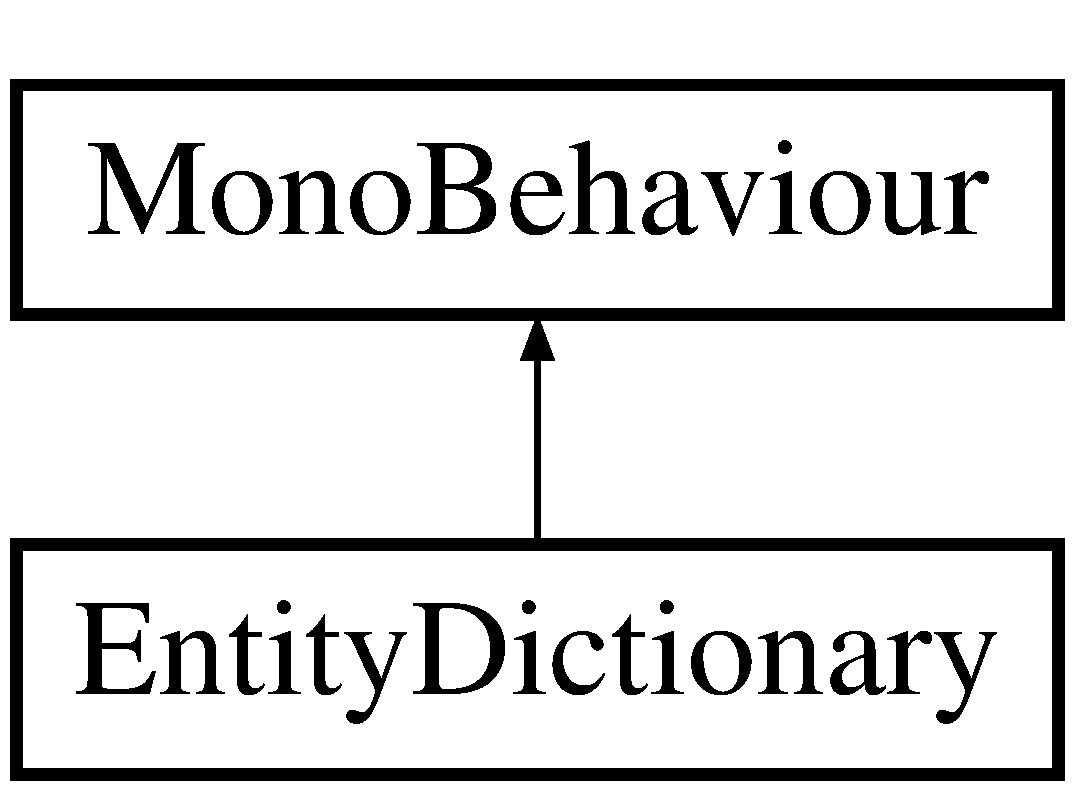
\includegraphics[height=2.000000cm]{class_entity_dictionary}
\end{center}
\end{figure}
\subsection*{Private Member Functions}
\begin{DoxyCompactItemize}
\item 
void \hyperlink{class_entity_dictionary_a592c626d86d178f69e9515a746c264d8}{Start} ()
\item 
void \hyperlink{class_entity_dictionary_a0d8b0d1c4b288bb0ec395f50816e9800}{Update} ()
\end{DoxyCompactItemize}


\subsection{Member Function Documentation}
\mbox{\Hypertarget{class_entity_dictionary_a592c626d86d178f69e9515a746c264d8}\label{class_entity_dictionary_a592c626d86d178f69e9515a746c264d8}} 
\index{Entity\+Dictionary@{Entity\+Dictionary}!Start@{Start}}
\index{Start@{Start}!Entity\+Dictionary@{Entity\+Dictionary}}
\subsubsection{\texorpdfstring{Start()}{Start()}}
{\footnotesize\ttfamily void Entity\+Dictionary.\+Start (\begin{DoxyParamCaption}{ }\end{DoxyParamCaption})\hspace{0.3cm}{\ttfamily [private]}}

\mbox{\Hypertarget{class_entity_dictionary_a0d8b0d1c4b288bb0ec395f50816e9800}\label{class_entity_dictionary_a0d8b0d1c4b288bb0ec395f50816e9800}} 
\index{Entity\+Dictionary@{Entity\+Dictionary}!Update@{Update}}
\index{Update@{Update}!Entity\+Dictionary@{Entity\+Dictionary}}
\subsubsection{\texorpdfstring{Update()}{Update()}}
{\footnotesize\ttfamily void Entity\+Dictionary.\+Update (\begin{DoxyParamCaption}{ }\end{DoxyParamCaption})\hspace{0.3cm}{\ttfamily [private]}}



The documentation for this class was generated from the following file\+:\begin{DoxyCompactItemize}
\item 
Assets/\hyperlink{_entity_dictionary_8cs}{Entity\+Dictionary.\+cs}\end{DoxyCompactItemize}

\hypertarget{class_entity_manager}{}\section{Entity\+Manager Class Reference}
\label{class_entity_manager}\index{Entity\+Manager@{Entity\+Manager}}
Inheritance diagram for Entity\+Manager\+:\begin{figure}[H]
\begin{center}
\leavevmode
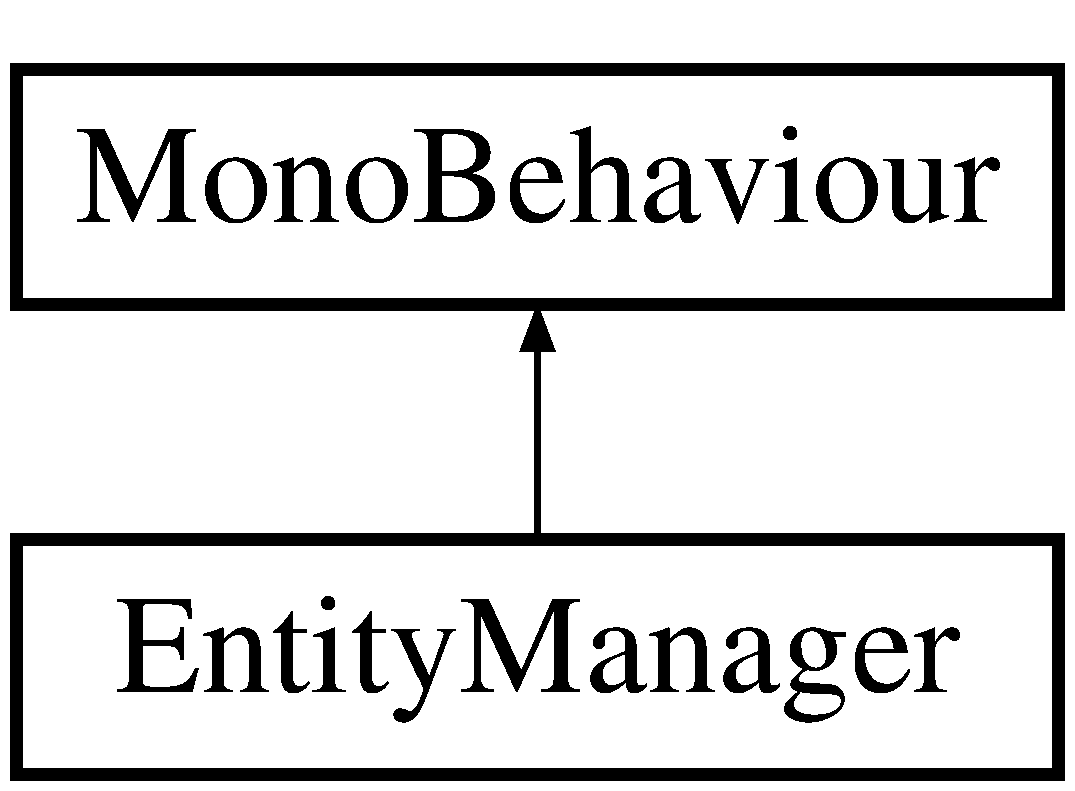
\includegraphics[height=2.000000cm]{class_entity_manager}
\end{center}
\end{figure}
\subsection*{Private Member Functions}
\begin{DoxyCompactItemize}
\item 
void \hyperlink{class_entity_manager_a3e72b6eace1b9c16b5267ca25a1e4fa8}{Start} ()
\item 
void \hyperlink{class_entity_manager_a842b748cc70c7e1366a57df0475b5b96}{Update} ()
\end{DoxyCompactItemize}
\subsection*{Private Attributes}
\begin{DoxyCompactItemize}
\item 
\hyperlink{class_entity_builder}{Entity\+Builder} \hyperlink{class_entity_manager_a0a1c610cd196c0832945dfd10009b18f}{m\+\_\+entity\+Builder}
\begin{DoxyCompactList}\small\item\em The builder class which \hyperlink{class_entity_manager}{Entity\+Manager} uses to get Entities. \end{DoxyCompactList}\end{DoxyCompactItemize}


\subsection{Member Function Documentation}
\mbox{\Hypertarget{class_entity_manager_a3e72b6eace1b9c16b5267ca25a1e4fa8}\label{class_entity_manager_a3e72b6eace1b9c16b5267ca25a1e4fa8}} 
\index{Entity\+Manager@{Entity\+Manager}!Start@{Start}}
\index{Start@{Start}!Entity\+Manager@{Entity\+Manager}}
\subsubsection{\texorpdfstring{Start()}{Start()}}
{\footnotesize\ttfamily void Entity\+Manager.\+Start (\begin{DoxyParamCaption}{ }\end{DoxyParamCaption})\hspace{0.3cm}{\ttfamily [private]}}

\mbox{\Hypertarget{class_entity_manager_a842b748cc70c7e1366a57df0475b5b96}\label{class_entity_manager_a842b748cc70c7e1366a57df0475b5b96}} 
\index{Entity\+Manager@{Entity\+Manager}!Update@{Update}}
\index{Update@{Update}!Entity\+Manager@{Entity\+Manager}}
\subsubsection{\texorpdfstring{Update()}{Update()}}
{\footnotesize\ttfamily void Entity\+Manager.\+Update (\begin{DoxyParamCaption}{ }\end{DoxyParamCaption})\hspace{0.3cm}{\ttfamily [private]}}



\subsection{Member Data Documentation}
\mbox{\Hypertarget{class_entity_manager_a0a1c610cd196c0832945dfd10009b18f}\label{class_entity_manager_a0a1c610cd196c0832945dfd10009b18f}} 
\index{Entity\+Manager@{Entity\+Manager}!m\+\_\+entity\+Builder@{m\+\_\+entity\+Builder}}
\index{m\+\_\+entity\+Builder@{m\+\_\+entity\+Builder}!Entity\+Manager@{Entity\+Manager}}
\subsubsection{\texorpdfstring{m\+\_\+entity\+Builder}{m\_entityBuilder}}
{\footnotesize\ttfamily \hyperlink{class_entity_builder}{Entity\+Builder} Entity\+Manager.\+m\+\_\+entity\+Builder\hspace{0.3cm}{\ttfamily [private]}}



The builder class which \hyperlink{class_entity_manager}{Entity\+Manager} uses to get Entities. 



The documentation for this class was generated from the following file\+:\begin{DoxyCompactItemize}
\item 
Assets/\hyperlink{_entity_manager_8cs}{Entity\+Manager.\+cs}\end{DoxyCompactItemize}

\hypertarget{class_enumerations}{}\section{Enumerations Class Reference}
\label{class_enumerations}\index{Enumerations@{Enumerations}}
\subsection*{Public Types}
\begin{DoxyCompactItemize}
\item 
enum \hyperlink{class_enumerations_a3822629637240e477854c9552d693417}{Entity\+Types} \{ \hyperlink{class_enumerations_a3822629637240e477854c9552d693417ac1bb19b27818343c1926119b958741b5}{Entity\+Types.\+Human} = 0, 
\hyperlink{class_enumerations_a3822629637240e477854c9552d693417a161e7ce7bfdc89ab4b9f52c1d4c94212}{Entity\+Types.\+Animal} = 1, 
\hyperlink{class_enumerations_a3822629637240e477854c9552d693417aaebfe46795575772b7cf413e25caeab9}{Entity\+Types.\+House} = 2
 \}\begin{DoxyCompactList}\small\item\em Enumeration to support selection of entity types for methods. \end{DoxyCompactList}
\item 
enum \hyperlink{class_enumerations_ae4fb3bfedbf076bc31c8939baac88745}{Landscape\+Types} \{ \hyperlink{class_enumerations_ae4fb3bfedbf076bc31c8939baac88745a149529f6dcbcc198787e69a11235422e}{Landscape\+Types.\+River} = 0, 
\hyperlink{class_enumerations_ae4fb3bfedbf076bc31c8939baac88745aec9903c79dd510ffa43f69ee867a9002}{Landscape\+Types.\+Mountain} = 1, 
\hyperlink{class_enumerations_ae4fb3bfedbf076bc31c8939baac88745a4cd8413207629a963225f4314b53adcd}{Landscape\+Types.\+Plain} = 2, 
\hyperlink{class_enumerations_ae4fb3bfedbf076bc31c8939baac88745aac12ee4aedb176eb73ce3f6c0d1e9036}{Landscape\+Types.\+Forest} = 3
 \}\begin{DoxyCompactList}\small\item\em Enumeration to support selection of entity types for methods. \end{DoxyCompactList}
\end{DoxyCompactItemize}


\subsection{Member Enumeration Documentation}
\mbox{\Hypertarget{class_enumerations_a3822629637240e477854c9552d693417}\label{class_enumerations_a3822629637240e477854c9552d693417}} 
\index{Enumerations@{Enumerations}!Entity\+Types@{Entity\+Types}}
\index{Entity\+Types@{Entity\+Types}!Enumerations@{Enumerations}}
\subsubsection{\texorpdfstring{Entity\+Types}{EntityTypes}}
{\footnotesize\ttfamily enum \hyperlink{class_enumerations_a3822629637240e477854c9552d693417}{Enumerations.\+Entity\+Types}\hspace{0.3cm}{\ttfamily [strong]}}



Enumeration to support selection of entity types for methods. 

\begin{DoxyEnumFields}{Enumerator}
\raisebox{\heightof{T}}[0pt][0pt]{\index{Human@{Human}!Enumerations@{Enumerations}}\index{Enumerations@{Enumerations}!Human@{Human}}}\mbox{\Hypertarget{class_enumerations_a3822629637240e477854c9552d693417ac1bb19b27818343c1926119b958741b5}\label{class_enumerations_a3822629637240e477854c9552d693417ac1bb19b27818343c1926119b958741b5}} 
Human&\\
\hline

\raisebox{\heightof{T}}[0pt][0pt]{\index{Animal@{Animal}!Enumerations@{Enumerations}}\index{Enumerations@{Enumerations}!Animal@{Animal}}}\mbox{\Hypertarget{class_enumerations_a3822629637240e477854c9552d693417a161e7ce7bfdc89ab4b9f52c1d4c94212}\label{class_enumerations_a3822629637240e477854c9552d693417a161e7ce7bfdc89ab4b9f52c1d4c94212}} 
Animal&\\
\hline

\raisebox{\heightof{T}}[0pt][0pt]{\index{House@{House}!Enumerations@{Enumerations}}\index{Enumerations@{Enumerations}!House@{House}}}\mbox{\Hypertarget{class_enumerations_a3822629637240e477854c9552d693417aaebfe46795575772b7cf413e25caeab9}\label{class_enumerations_a3822629637240e477854c9552d693417aaebfe46795575772b7cf413e25caeab9}} 
House&\\
\hline

\end{DoxyEnumFields}
\mbox{\Hypertarget{class_enumerations_ae4fb3bfedbf076bc31c8939baac88745}\label{class_enumerations_ae4fb3bfedbf076bc31c8939baac88745}} 
\index{Enumerations@{Enumerations}!Landscape\+Types@{Landscape\+Types}}
\index{Landscape\+Types@{Landscape\+Types}!Enumerations@{Enumerations}}
\subsubsection{\texorpdfstring{Landscape\+Types}{LandscapeTypes}}
{\footnotesize\ttfamily enum \hyperlink{class_enumerations_ae4fb3bfedbf076bc31c8939baac88745}{Enumerations.\+Landscape\+Types}\hspace{0.3cm}{\ttfamily [strong]}}



Enumeration to support selection of entity types for methods. 

\begin{DoxyEnumFields}{Enumerator}
\raisebox{\heightof{T}}[0pt][0pt]{\index{River@{River}!Enumerations@{Enumerations}}\index{Enumerations@{Enumerations}!River@{River}}}\mbox{\Hypertarget{class_enumerations_ae4fb3bfedbf076bc31c8939baac88745a149529f6dcbcc198787e69a11235422e}\label{class_enumerations_ae4fb3bfedbf076bc31c8939baac88745a149529f6dcbcc198787e69a11235422e}} 
River&\\
\hline

\raisebox{\heightof{T}}[0pt][0pt]{\index{Mountain@{Mountain}!Enumerations@{Enumerations}}\index{Enumerations@{Enumerations}!Mountain@{Mountain}}}\mbox{\Hypertarget{class_enumerations_ae4fb3bfedbf076bc31c8939baac88745aec9903c79dd510ffa43f69ee867a9002}\label{class_enumerations_ae4fb3bfedbf076bc31c8939baac88745aec9903c79dd510ffa43f69ee867a9002}} 
Mountain&\\
\hline

\raisebox{\heightof{T}}[0pt][0pt]{\index{Plain@{Plain}!Enumerations@{Enumerations}}\index{Enumerations@{Enumerations}!Plain@{Plain}}}\mbox{\Hypertarget{class_enumerations_ae4fb3bfedbf076bc31c8939baac88745a4cd8413207629a963225f4314b53adcd}\label{class_enumerations_ae4fb3bfedbf076bc31c8939baac88745a4cd8413207629a963225f4314b53adcd}} 
Plain&\\
\hline

\raisebox{\heightof{T}}[0pt][0pt]{\index{Forest@{Forest}!Enumerations@{Enumerations}}\index{Enumerations@{Enumerations}!Forest@{Forest}}}\mbox{\Hypertarget{class_enumerations_ae4fb3bfedbf076bc31c8939baac88745aac12ee4aedb176eb73ce3f6c0d1e9036}\label{class_enumerations_ae4fb3bfedbf076bc31c8939baac88745aac12ee4aedb176eb73ce3f6c0d1e9036}} 
Forest&\\
\hline

\end{DoxyEnumFields}


The documentation for this class was generated from the following file\+:\begin{DoxyCompactItemize}
\item 
Assets/\hyperlink{_enumerations_8cs}{Enumerations.\+cs}\end{DoxyCompactItemize}

\hypertarget{class_first_person_camera}{}\section{First\+Person\+Camera Class Reference}
\label{class_first_person_camera}\index{First\+Person\+Camera@{First\+Person\+Camera}}
Inheritance diagram for First\+Person\+Camera\+:\begin{figure}[H]
\begin{center}
\leavevmode
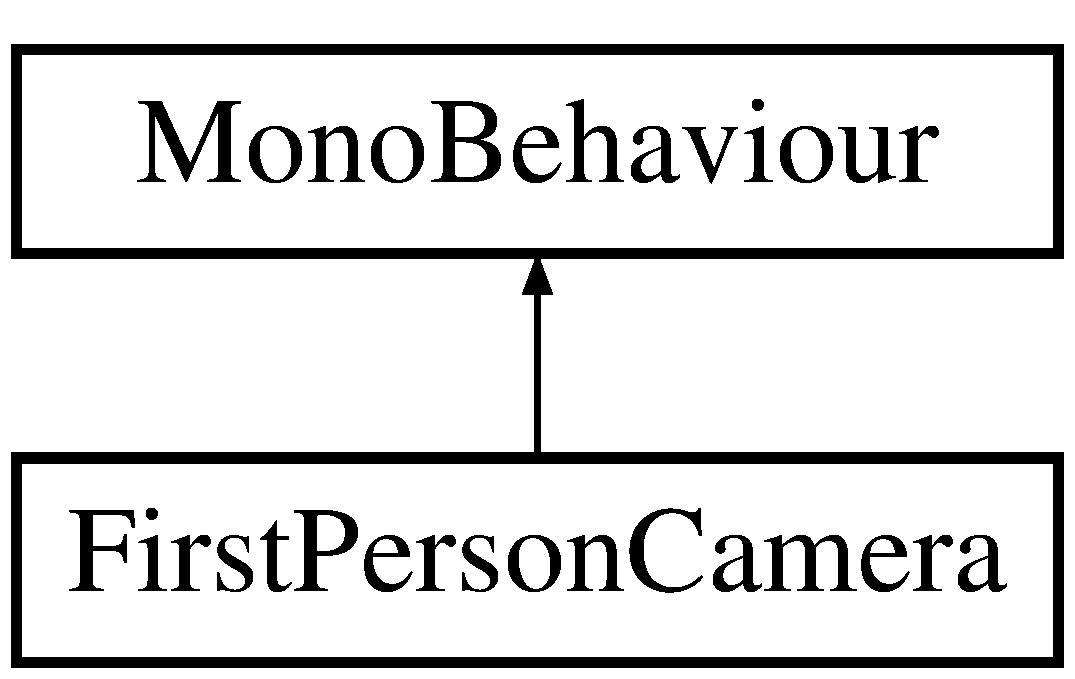
\includegraphics[height=2.000000cm]{class_first_person_camera}
\end{center}
\end{figure}
\subsection*{Private Member Functions}
\begin{DoxyCompactItemize}
\item 
void \hyperlink{class_first_person_camera_a78e3e8f10a7ed9b250b656da3dddeda8}{Start} ()
\item 
void \hyperlink{class_first_person_camera_a0f4eab1db8fc0b912ca0858b9e723110}{Update} ()
\end{DoxyCompactItemize}


\subsection{Member Function Documentation}
\mbox{\Hypertarget{class_first_person_camera_a78e3e8f10a7ed9b250b656da3dddeda8}\label{class_first_person_camera_a78e3e8f10a7ed9b250b656da3dddeda8}} 
\index{First\+Person\+Camera@{First\+Person\+Camera}!Start@{Start}}
\index{Start@{Start}!First\+Person\+Camera@{First\+Person\+Camera}}
\subsubsection{\texorpdfstring{Start()}{Start()}}
{\footnotesize\ttfamily void First\+Person\+Camera.\+Start (\begin{DoxyParamCaption}{ }\end{DoxyParamCaption})\hspace{0.3cm}{\ttfamily [private]}}

\mbox{\Hypertarget{class_first_person_camera_a0f4eab1db8fc0b912ca0858b9e723110}\label{class_first_person_camera_a0f4eab1db8fc0b912ca0858b9e723110}} 
\index{First\+Person\+Camera@{First\+Person\+Camera}!Update@{Update}}
\index{Update@{Update}!First\+Person\+Camera@{First\+Person\+Camera}}
\subsubsection{\texorpdfstring{Update()}{Update()}}
{\footnotesize\ttfamily void First\+Person\+Camera.\+Update (\begin{DoxyParamCaption}{ }\end{DoxyParamCaption})\hspace{0.3cm}{\ttfamily [private]}}



The documentation for this class was generated from the following file\+:\begin{DoxyCompactItemize}
\item 
Assets/\hyperlink{_first_person_camera_8cs}{First\+Person\+Camera.\+cs}\end{DoxyCompactItemize}

\hypertarget{class_forest}{}\section{Forest Class Reference}
\label{class_forest}\index{Forest@{Forest}}
Inheritance diagram for Forest\+:\begin{figure}[H]
\begin{center}
\leavevmode
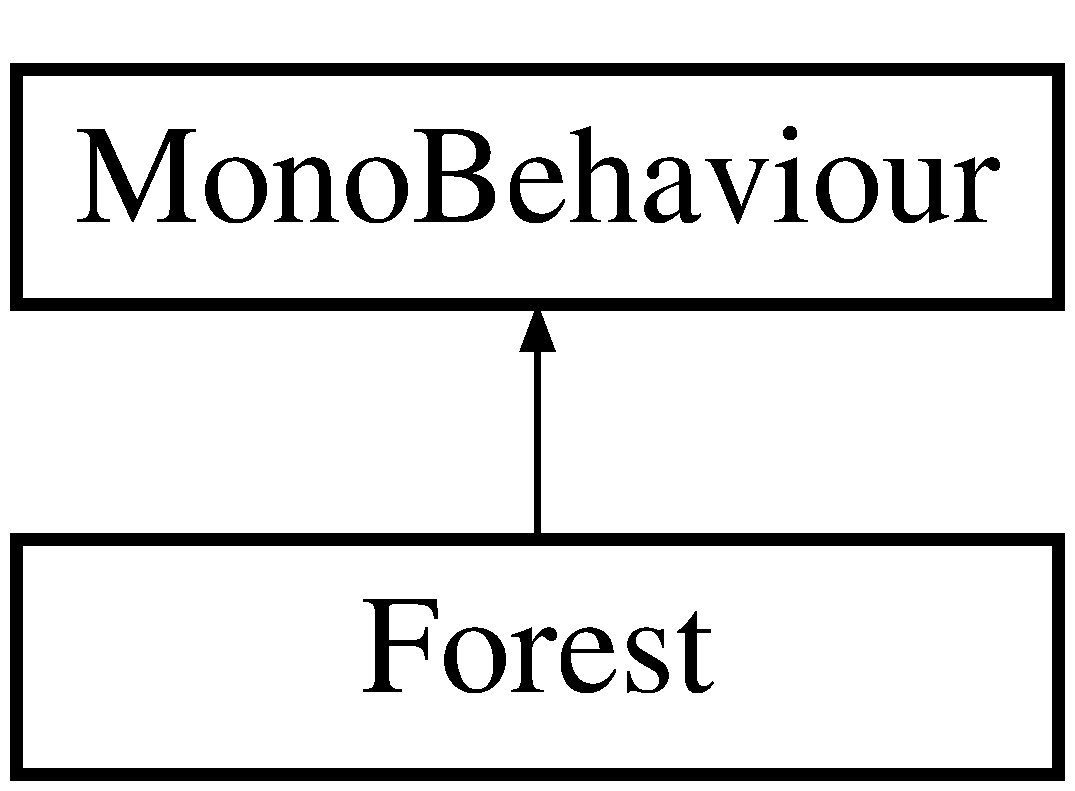
\includegraphics[height=2.000000cm]{class_forest}
\end{center}
\end{figure}
\subsection*{Private Member Functions}
\begin{DoxyCompactItemize}
\item 
void \hyperlink{class_forest_a25458c04d7b7e9c8920afc789434662e}{Start} ()
\item 
void \hyperlink{class_forest_a62b569afc7e204e1cb3015256060fb0d}{Update} ()
\end{DoxyCompactItemize}


\subsection{Member Function Documentation}
\mbox{\Hypertarget{class_forest_a25458c04d7b7e9c8920afc789434662e}\label{class_forest_a25458c04d7b7e9c8920afc789434662e}} 
\index{Forest@{Forest}!Start@{Start}}
\index{Start@{Start}!Forest@{Forest}}
\subsubsection{\texorpdfstring{Start()}{Start()}}
{\footnotesize\ttfamily void Forest.\+Start (\begin{DoxyParamCaption}{ }\end{DoxyParamCaption})\hspace{0.3cm}{\ttfamily [private]}}

\mbox{\Hypertarget{class_forest_a62b569afc7e204e1cb3015256060fb0d}\label{class_forest_a62b569afc7e204e1cb3015256060fb0d}} 
\index{Forest@{Forest}!Update@{Update}}
\index{Update@{Update}!Forest@{Forest}}
\subsubsection{\texorpdfstring{Update()}{Update()}}
{\footnotesize\ttfamily void Forest.\+Update (\begin{DoxyParamCaption}{ }\end{DoxyParamCaption})\hspace{0.3cm}{\ttfamily [private]}}



The documentation for this class was generated from the following file\+:\begin{DoxyCompactItemize}
\item 
Assets/\hyperlink{_forest_8cs}{Forest.\+cs}\end{DoxyCompactItemize}

\hypertarget{class_graphic}{}\section{Graphic Class Reference}
\label{class_graphic}\index{Graphic@{Graphic}}
Inheritance diagram for Graphic\+:\begin{figure}[H]
\begin{center}
\leavevmode
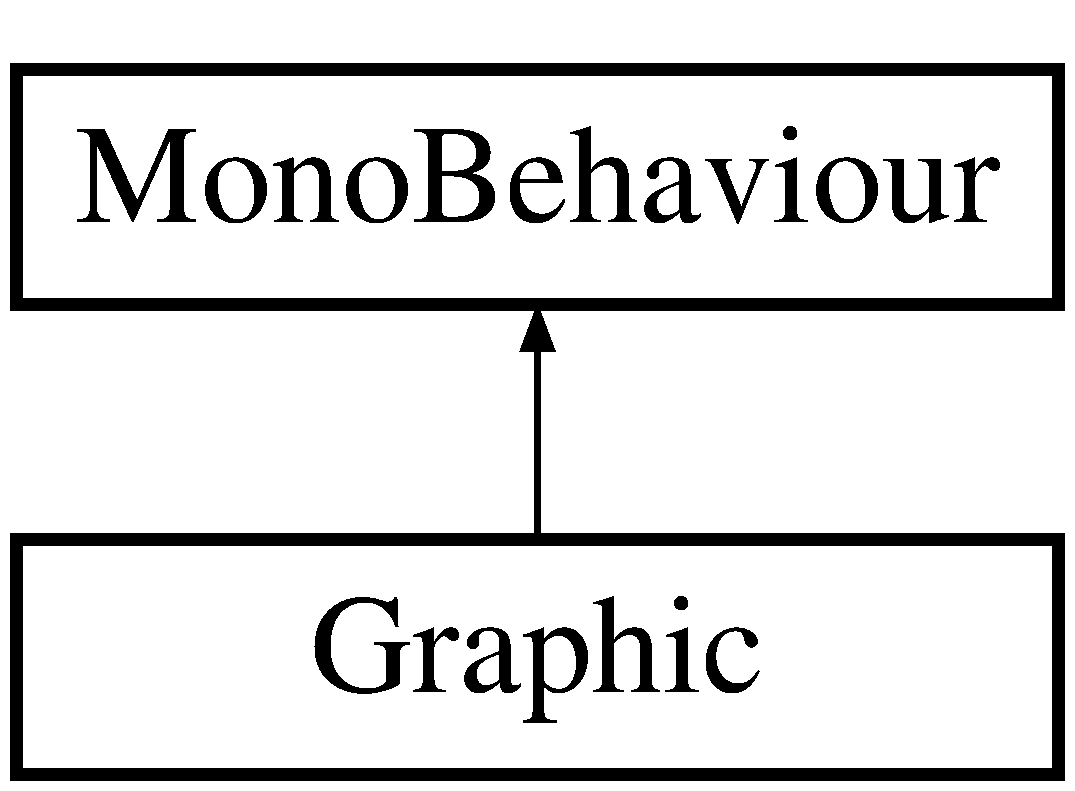
\includegraphics[height=2.000000cm]{class_graphic}
\end{center}
\end{figure}
\subsection*{Private Member Functions}
\begin{DoxyCompactItemize}
\item 
void \hyperlink{class_graphic_a382da4af4932b2aaffec2d5083527fbd}{Start} ()
\item 
void \hyperlink{class_graphic_a6d4e14e5b088fdffe79fe221ca2f2a10}{Update} ()
\end{DoxyCompactItemize}


\subsection{Member Function Documentation}
\mbox{\Hypertarget{class_graphic_a382da4af4932b2aaffec2d5083527fbd}\label{class_graphic_a382da4af4932b2aaffec2d5083527fbd}} 
\index{Graphic@{Graphic}!Start@{Start}}
\index{Start@{Start}!Graphic@{Graphic}}
\subsubsection{\texorpdfstring{Start()}{Start()}}
{\footnotesize\ttfamily void Graphic.\+Start (\begin{DoxyParamCaption}{ }\end{DoxyParamCaption})\hspace{0.3cm}{\ttfamily [private]}}

\mbox{\Hypertarget{class_graphic_a6d4e14e5b088fdffe79fe221ca2f2a10}\label{class_graphic_a6d4e14e5b088fdffe79fe221ca2f2a10}} 
\index{Graphic@{Graphic}!Update@{Update}}
\index{Update@{Update}!Graphic@{Graphic}}
\subsubsection{\texorpdfstring{Update()}{Update()}}
{\footnotesize\ttfamily void Graphic.\+Update (\begin{DoxyParamCaption}{ }\end{DoxyParamCaption})\hspace{0.3cm}{\ttfamily [private]}}



The documentation for this class was generated from the following file\+:\begin{DoxyCompactItemize}
\item 
Assets/\hyperlink{_graphic_8cs}{Graphic.\+cs}\end{DoxyCompactItemize}

\hypertarget{class_house}{}\section{House Class Reference}
\label{class_house}\index{House@{House}}
Inheritance diagram for House\+:\begin{figure}[H]
\begin{center}
\leavevmode
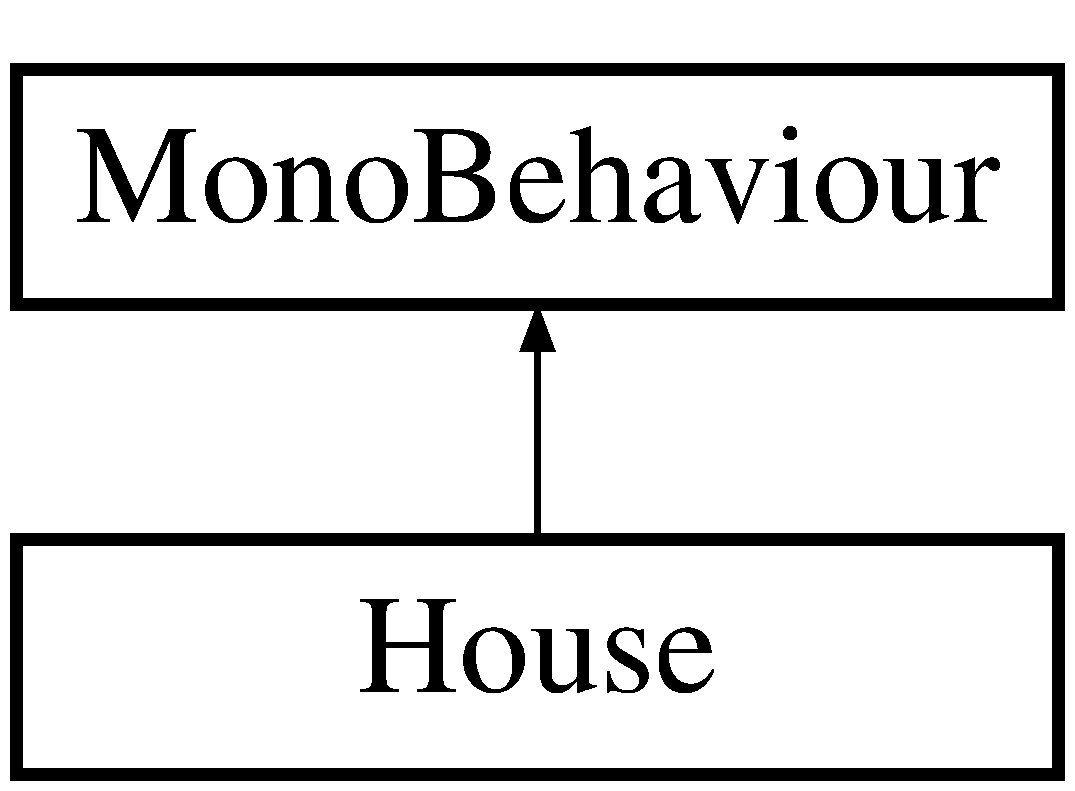
\includegraphics[height=2.000000cm]{class_house}
\end{center}
\end{figure}
\subsection*{Private Member Functions}
\begin{DoxyCompactItemize}
\item 
void \hyperlink{class_house_a15ab6066a77137144da99a8d721fe4e8}{Start} ()
\item 
void \hyperlink{class_house_a685c74a84fbe4dce8482be9cff0a43b8}{Update} ()
\end{DoxyCompactItemize}


\subsection{Member Function Documentation}
\mbox{\Hypertarget{class_house_a15ab6066a77137144da99a8d721fe4e8}\label{class_house_a15ab6066a77137144da99a8d721fe4e8}} 
\index{House@{House}!Start@{Start}}
\index{Start@{Start}!House@{House}}
\subsubsection{\texorpdfstring{Start()}{Start()}}
{\footnotesize\ttfamily void House.\+Start (\begin{DoxyParamCaption}{ }\end{DoxyParamCaption})\hspace{0.3cm}{\ttfamily [private]}}

\mbox{\Hypertarget{class_house_a685c74a84fbe4dce8482be9cff0a43b8}\label{class_house_a685c74a84fbe4dce8482be9cff0a43b8}} 
\index{House@{House}!Update@{Update}}
\index{Update@{Update}!House@{House}}
\subsubsection{\texorpdfstring{Update()}{Update()}}
{\footnotesize\ttfamily void House.\+Update (\begin{DoxyParamCaption}{ }\end{DoxyParamCaption})\hspace{0.3cm}{\ttfamily [private]}}



The documentation for this class was generated from the following file\+:\begin{DoxyCompactItemize}
\item 
Assets/\hyperlink{_house_8cs}{House.\+cs}\end{DoxyCompactItemize}

\hypertarget{class_human}{}\section{Human Class Reference}
\label{class_human}\index{Human@{Human}}
Inheritance diagram for Human\+:\begin{figure}[H]
\begin{center}
\leavevmode
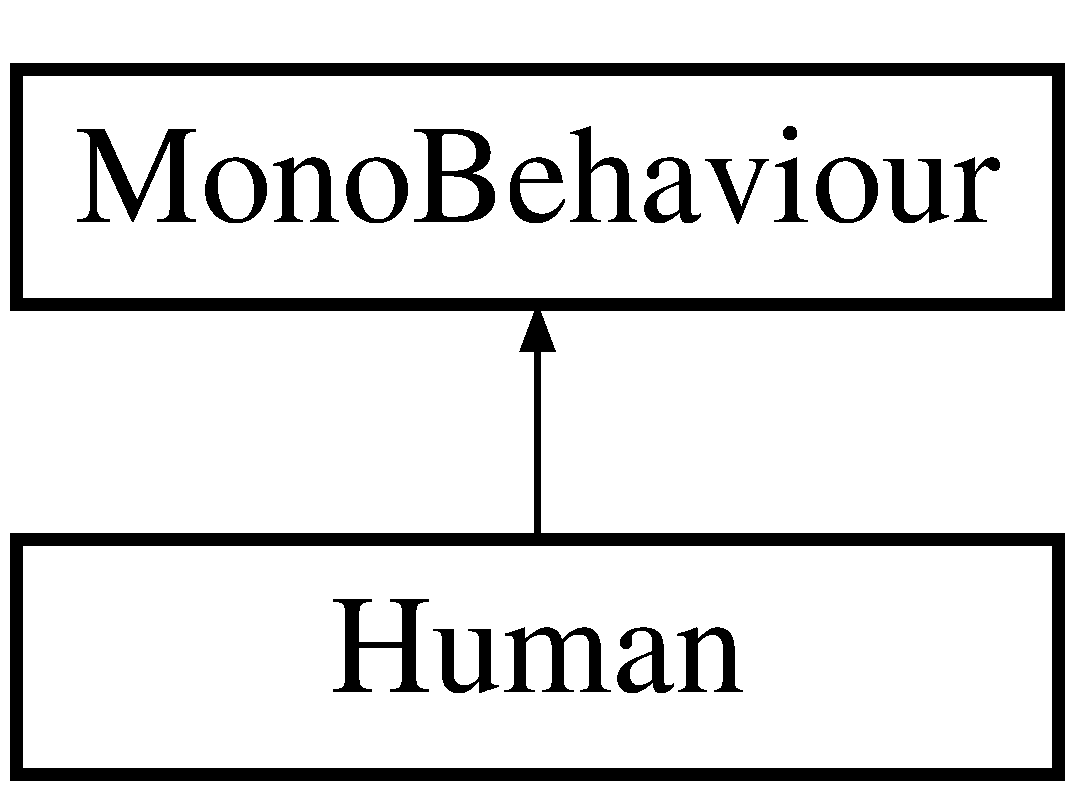
\includegraphics[height=2.000000cm]{class_human}
\end{center}
\end{figure}
\subsection*{Private Member Functions}
\begin{DoxyCompactItemize}
\item 
void \hyperlink{class_human_ad90a5e6e13a58f4340825d16a75afcf6}{Start} ()
\item 
void \hyperlink{class_human_a615b9b36e637a70156b748fc56c64b84}{Update} ()
\end{DoxyCompactItemize}


\subsection{Member Function Documentation}
\mbox{\Hypertarget{class_human_ad90a5e6e13a58f4340825d16a75afcf6}\label{class_human_ad90a5e6e13a58f4340825d16a75afcf6}} 
\index{Human@{Human}!Start@{Start}}
\index{Start@{Start}!Human@{Human}}
\subsubsection{\texorpdfstring{Start()}{Start()}}
{\footnotesize\ttfamily void Human.\+Start (\begin{DoxyParamCaption}{ }\end{DoxyParamCaption})\hspace{0.3cm}{\ttfamily [private]}}

\mbox{\Hypertarget{class_human_a615b9b36e637a70156b748fc56c64b84}\label{class_human_a615b9b36e637a70156b748fc56c64b84}} 
\index{Human@{Human}!Update@{Update}}
\index{Update@{Update}!Human@{Human}}
\subsubsection{\texorpdfstring{Update()}{Update()}}
{\footnotesize\ttfamily void Human.\+Update (\begin{DoxyParamCaption}{ }\end{DoxyParamCaption})\hspace{0.3cm}{\ttfamily [private]}}



The documentation for this class was generated from the following file\+:\begin{DoxyCompactItemize}
\item 
Assets/\hyperlink{_human_8cs}{Human.\+cs}\end{DoxyCompactItemize}

\hypertarget{class_input_manager}{}\section{Input\+Manager Class Reference}
\label{class_input_manager}\index{Input\+Manager@{Input\+Manager}}
Inheritance diagram for Input\+Manager\+:\begin{figure}[H]
\begin{center}
\leavevmode
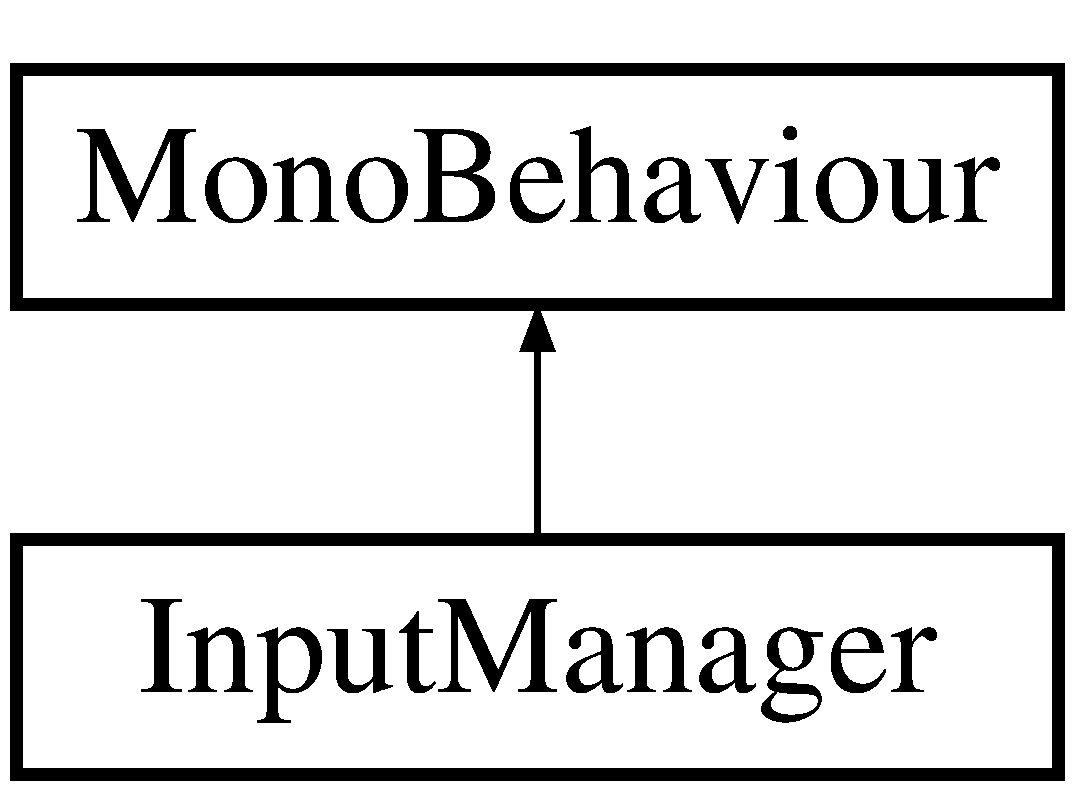
\includegraphics[height=2.000000cm]{class_input_manager}
\end{center}
\end{figure}
\subsection*{Private Member Functions}
\begin{DoxyCompactItemize}
\item 
void \hyperlink{class_input_manager_a5ea91a2053e03c49da58ee3a56628763}{Start} ()
\item 
void \hyperlink{class_input_manager_a17a33be75084fed42bebb52892323c62}{Update} ()
\end{DoxyCompactItemize}


\subsection{Member Function Documentation}
\mbox{\Hypertarget{class_input_manager_a5ea91a2053e03c49da58ee3a56628763}\label{class_input_manager_a5ea91a2053e03c49da58ee3a56628763}} 
\index{Input\+Manager@{Input\+Manager}!Start@{Start}}
\index{Start@{Start}!Input\+Manager@{Input\+Manager}}
\subsubsection{\texorpdfstring{Start()}{Start()}}
{\footnotesize\ttfamily void Input\+Manager.\+Start (\begin{DoxyParamCaption}{ }\end{DoxyParamCaption})\hspace{0.3cm}{\ttfamily [private]}}

\mbox{\Hypertarget{class_input_manager_a17a33be75084fed42bebb52892323c62}\label{class_input_manager_a17a33be75084fed42bebb52892323c62}} 
\index{Input\+Manager@{Input\+Manager}!Update@{Update}}
\index{Update@{Update}!Input\+Manager@{Input\+Manager}}
\subsubsection{\texorpdfstring{Update()}{Update()}}
{\footnotesize\ttfamily void Input\+Manager.\+Update (\begin{DoxyParamCaption}{ }\end{DoxyParamCaption})\hspace{0.3cm}{\ttfamily [private]}}



The documentation for this class was generated from the following file\+:\begin{DoxyCompactItemize}
\item 
Assets/\hyperlink{_input_manager_8cs}{Input\+Manager.\+cs}\end{DoxyCompactItemize}

\hypertarget{class_isometric_camera}{}\section{Isometric\+Camera Class Reference}
\label{class_isometric_camera}\index{Isometric\+Camera@{Isometric\+Camera}}
Inheritance diagram for Isometric\+Camera\+:\begin{figure}[H]
\begin{center}
\leavevmode
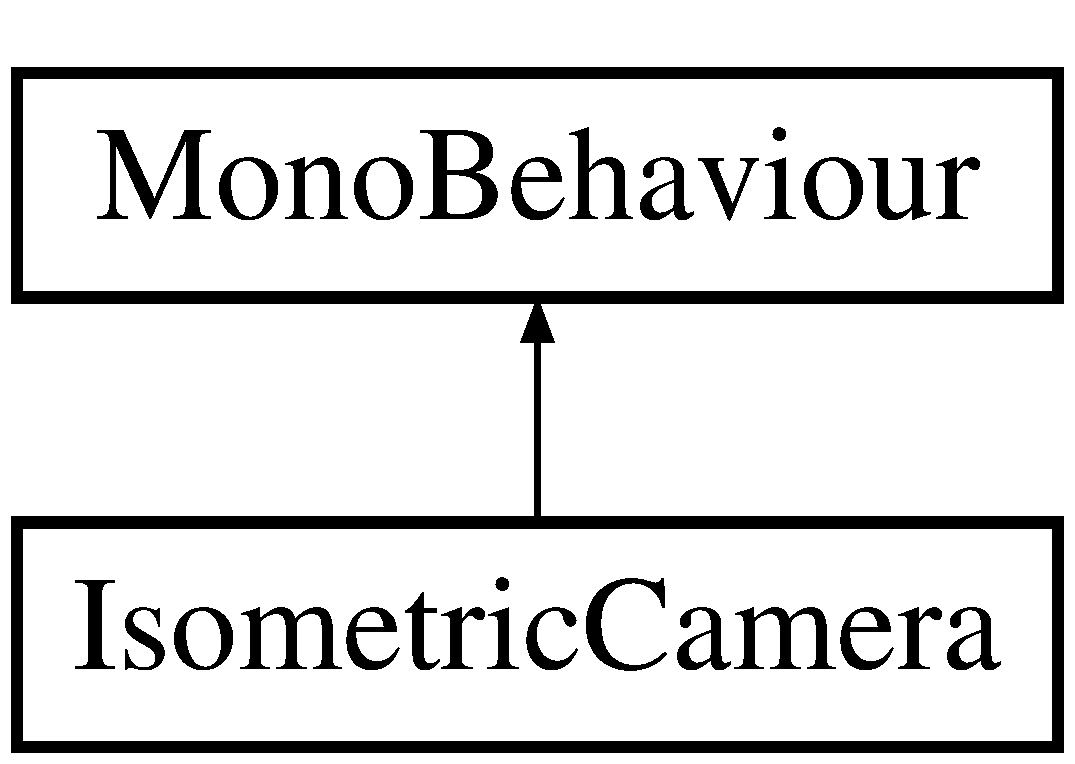
\includegraphics[height=2.000000cm]{class_isometric_camera}
\end{center}
\end{figure}
\subsection*{Private Member Functions}
\begin{DoxyCompactItemize}
\item 
void \hyperlink{class_isometric_camera_abab67ea7f8d0ac64cb4cea6237a1b171}{Start} ()
\item 
void \hyperlink{class_isometric_camera_a85478a65a084183529f08b390ac9180b}{Update} ()
\end{DoxyCompactItemize}


\subsection{Member Function Documentation}
\mbox{\Hypertarget{class_isometric_camera_abab67ea7f8d0ac64cb4cea6237a1b171}\label{class_isometric_camera_abab67ea7f8d0ac64cb4cea6237a1b171}} 
\index{Isometric\+Camera@{Isometric\+Camera}!Start@{Start}}
\index{Start@{Start}!Isometric\+Camera@{Isometric\+Camera}}
\subsubsection{\texorpdfstring{Start()}{Start()}}
{\footnotesize\ttfamily void Isometric\+Camera.\+Start (\begin{DoxyParamCaption}{ }\end{DoxyParamCaption})\hspace{0.3cm}{\ttfamily [private]}}

\mbox{\Hypertarget{class_isometric_camera_a85478a65a084183529f08b390ac9180b}\label{class_isometric_camera_a85478a65a084183529f08b390ac9180b}} 
\index{Isometric\+Camera@{Isometric\+Camera}!Update@{Update}}
\index{Update@{Update}!Isometric\+Camera@{Isometric\+Camera}}
\subsubsection{\texorpdfstring{Update()}{Update()}}
{\footnotesize\ttfamily void Isometric\+Camera.\+Update (\begin{DoxyParamCaption}{ }\end{DoxyParamCaption})\hspace{0.3cm}{\ttfamily [private]}}



The documentation for this class was generated from the following file\+:\begin{DoxyCompactItemize}
\item 
Assets/\hyperlink{_isometric_camera_8cs}{Isometric\+Camera.\+cs}\end{DoxyCompactItemize}

\hypertarget{class_landscape}{}\section{Landscape Class Reference}
\label{class_landscape}\index{Landscape@{Landscape}}
Inheritance diagram for Landscape\+:\begin{figure}[H]
\begin{center}
\leavevmode
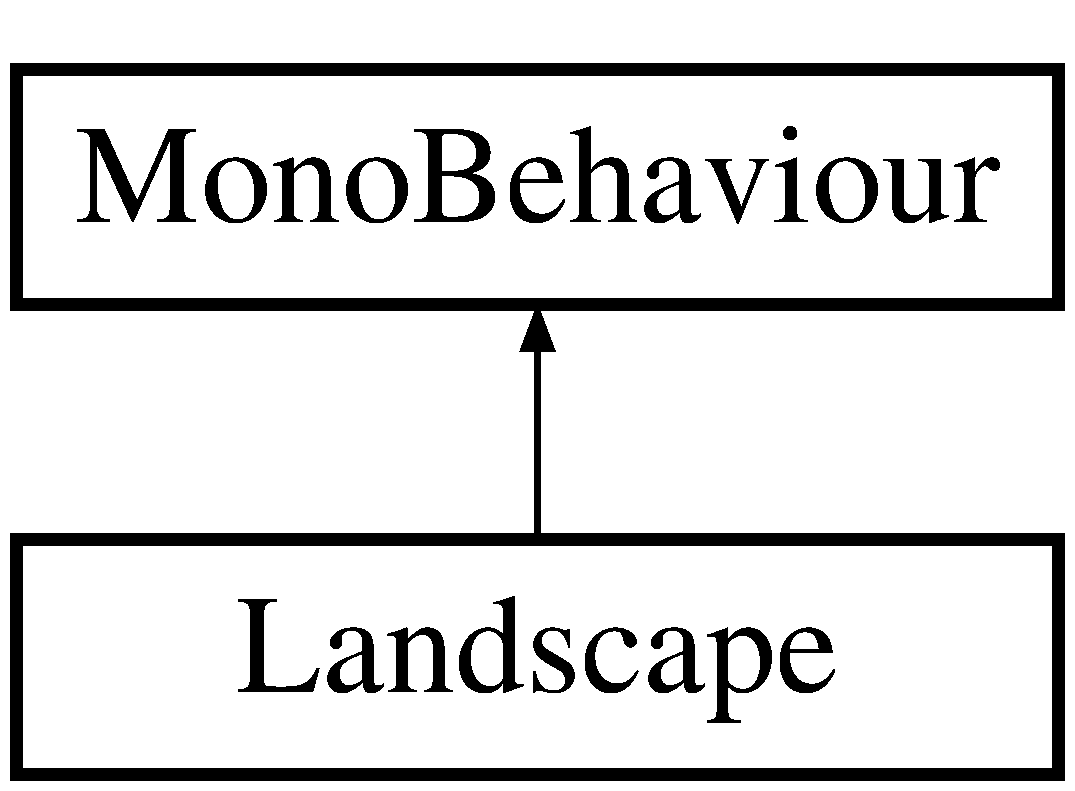
\includegraphics[height=2.000000cm]{class_landscape}
\end{center}
\end{figure}
\subsection*{Private Member Functions}
\begin{DoxyCompactItemize}
\item 
void \hyperlink{class_landscape_ad60d989f987193736801f9d3b0ffd126}{Start} ()
\item 
void \hyperlink{class_landscape_a2c6abdd5528abe96365f1abe0b0c394f}{Update} ()
\end{DoxyCompactItemize}


\subsection{Member Function Documentation}
\mbox{\Hypertarget{class_landscape_ad60d989f987193736801f9d3b0ffd126}\label{class_landscape_ad60d989f987193736801f9d3b0ffd126}} 
\index{Landscape@{Landscape}!Start@{Start}}
\index{Start@{Start}!Landscape@{Landscape}}
\subsubsection{\texorpdfstring{Start()}{Start()}}
{\footnotesize\ttfamily void Landscape.\+Start (\begin{DoxyParamCaption}{ }\end{DoxyParamCaption})\hspace{0.3cm}{\ttfamily [private]}}

\mbox{\Hypertarget{class_landscape_a2c6abdd5528abe96365f1abe0b0c394f}\label{class_landscape_a2c6abdd5528abe96365f1abe0b0c394f}} 
\index{Landscape@{Landscape}!Update@{Update}}
\index{Update@{Update}!Landscape@{Landscape}}
\subsubsection{\texorpdfstring{Update()}{Update()}}
{\footnotesize\ttfamily void Landscape.\+Update (\begin{DoxyParamCaption}{ }\end{DoxyParamCaption})\hspace{0.3cm}{\ttfamily [private]}}



The documentation for this class was generated from the following file\+:\begin{DoxyCompactItemize}
\item 
Assets/\hyperlink{_landscape_8cs}{Landscape.\+cs}\end{DoxyCompactItemize}

\hypertarget{class_landscape_builder}{}\section{Landscape\+Builder Class Reference}
\label{class_landscape_builder}\index{Landscape\+Builder@{Landscape\+Builder}}
Inheritance diagram for Landscape\+Builder\+:\begin{figure}[H]
\begin{center}
\leavevmode
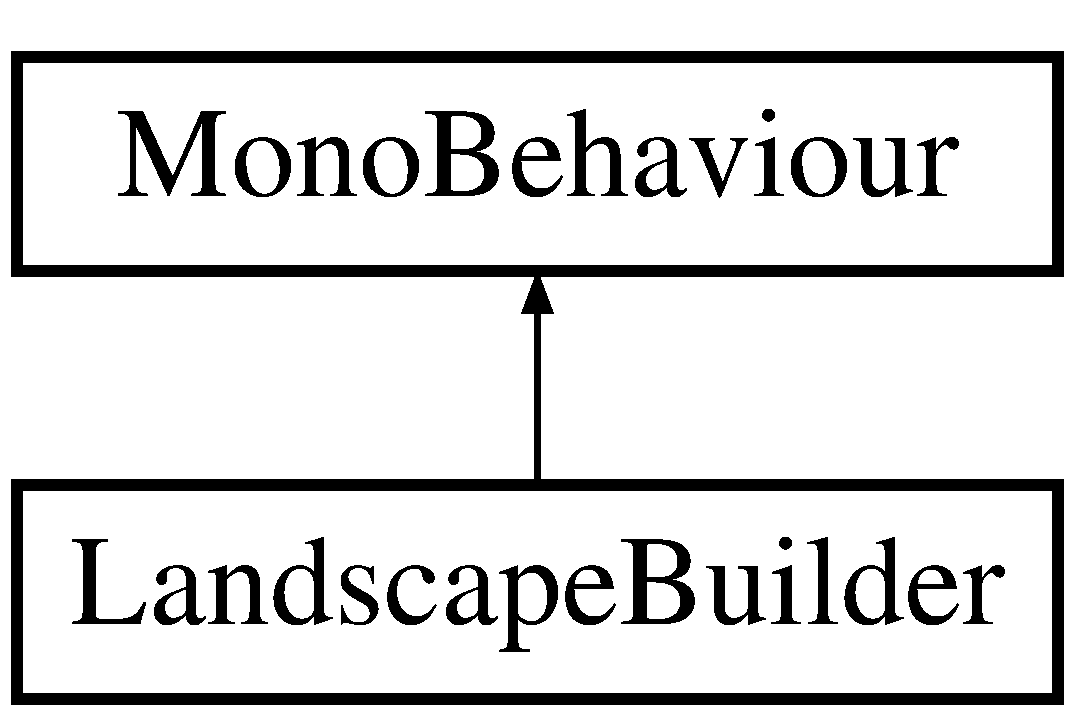
\includegraphics[height=2.000000cm]{class_landscape_builder}
\end{center}
\end{figure}
\subsection*{Private Member Functions}
\begin{DoxyCompactItemize}
\item 
void \hyperlink{class_landscape_builder_af6eb2a1ca1357aba9dbbf3ea13ef7a09}{Start} ()
\item 
void \hyperlink{class_landscape_builder_a117e41633ea31c2c25abce388a46465d}{Update} ()
\end{DoxyCompactItemize}
\subsection*{Private Attributes}
\begin{DoxyCompactItemize}
\item 
\hyperlink{class_landscape_dictionary}{Landscape\+Dictionary} \hyperlink{class_landscape_builder_ab732ac4dd39fe671a30e3a614a1c65b9}{m\+\_\+landscape\+Dictionary}
\begin{DoxyCompactList}\small\item\em The dictionary of methods by which \hyperlink{class_landscape_builder}{Landscape\+Builder} builds \hyperlink{class_landscape}{Landscape} objects. \end{DoxyCompactList}\end{DoxyCompactItemize}


\subsection{Member Function Documentation}
\mbox{\Hypertarget{class_landscape_builder_af6eb2a1ca1357aba9dbbf3ea13ef7a09}\label{class_landscape_builder_af6eb2a1ca1357aba9dbbf3ea13ef7a09}} 
\index{Landscape\+Builder@{Landscape\+Builder}!Start@{Start}}
\index{Start@{Start}!Landscape\+Builder@{Landscape\+Builder}}
\subsubsection{\texorpdfstring{Start()}{Start()}}
{\footnotesize\ttfamily void Landscape\+Builder.\+Start (\begin{DoxyParamCaption}{ }\end{DoxyParamCaption})\hspace{0.3cm}{\ttfamily [private]}}

\mbox{\Hypertarget{class_landscape_builder_a117e41633ea31c2c25abce388a46465d}\label{class_landscape_builder_a117e41633ea31c2c25abce388a46465d}} 
\index{Landscape\+Builder@{Landscape\+Builder}!Update@{Update}}
\index{Update@{Update}!Landscape\+Builder@{Landscape\+Builder}}
\subsubsection{\texorpdfstring{Update()}{Update()}}
{\footnotesize\ttfamily void Landscape\+Builder.\+Update (\begin{DoxyParamCaption}{ }\end{DoxyParamCaption})\hspace{0.3cm}{\ttfamily [private]}}



\subsection{Member Data Documentation}
\mbox{\Hypertarget{class_landscape_builder_ab732ac4dd39fe671a30e3a614a1c65b9}\label{class_landscape_builder_ab732ac4dd39fe671a30e3a614a1c65b9}} 
\index{Landscape\+Builder@{Landscape\+Builder}!m\+\_\+landscape\+Dictionary@{m\+\_\+landscape\+Dictionary}}
\index{m\+\_\+landscape\+Dictionary@{m\+\_\+landscape\+Dictionary}!Landscape\+Builder@{Landscape\+Builder}}
\subsubsection{\texorpdfstring{m\+\_\+landscape\+Dictionary}{m\_landscapeDictionary}}
{\footnotesize\ttfamily \hyperlink{class_landscape_dictionary}{Landscape\+Dictionary} Landscape\+Builder.\+m\+\_\+landscape\+Dictionary\hspace{0.3cm}{\ttfamily [private]}}



The dictionary of methods by which \hyperlink{class_landscape_builder}{Landscape\+Builder} builds \hyperlink{class_landscape}{Landscape} objects. 



The documentation for this class was generated from the following file\+:\begin{DoxyCompactItemize}
\item 
Assets/\hyperlink{_landscape_builder_8cs}{Landscape\+Builder.\+cs}\end{DoxyCompactItemize}

\hypertarget{class_landscape_dictionary}{}\section{Landscape\+Dictionary Class Reference}
\label{class_landscape_dictionary}\index{Landscape\+Dictionary@{Landscape\+Dictionary}}
Inheritance diagram for Landscape\+Dictionary\+:\begin{figure}[H]
\begin{center}
\leavevmode
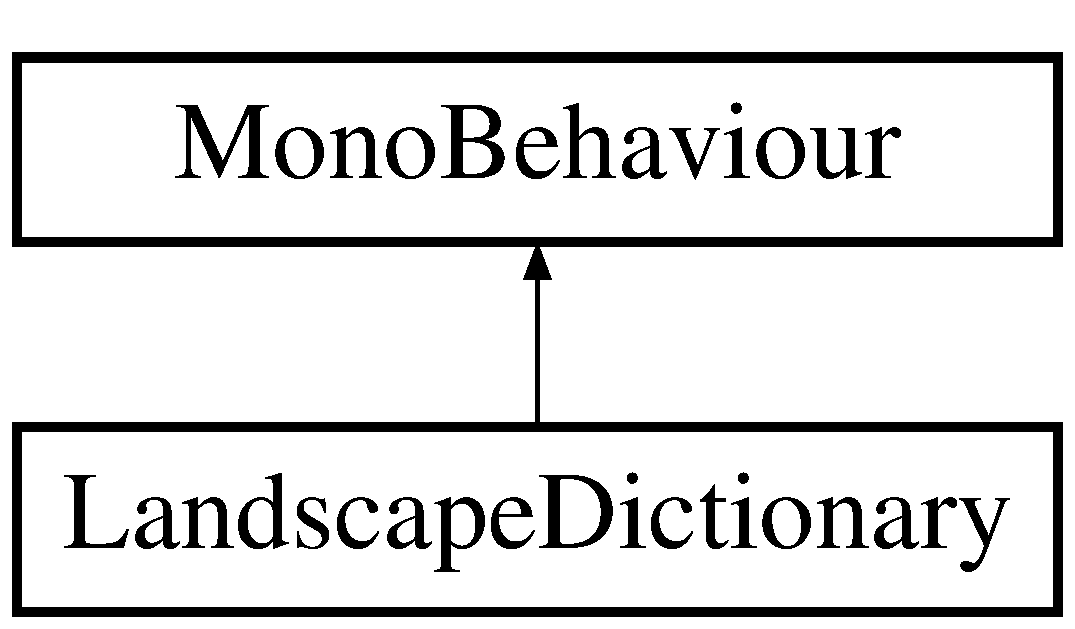
\includegraphics[height=2.000000cm]{class_landscape_dictionary}
\end{center}
\end{figure}
\subsection*{Private Member Functions}
\begin{DoxyCompactItemize}
\item 
void \hyperlink{class_landscape_dictionary_af7832ca835e7deea26761554ba3adf26}{Start} ()
\item 
void \hyperlink{class_landscape_dictionary_a7a8ccbe99b7a687d79fb34d32061c401}{Update} ()
\end{DoxyCompactItemize}


\subsection{Member Function Documentation}
\mbox{\Hypertarget{class_landscape_dictionary_af7832ca835e7deea26761554ba3adf26}\label{class_landscape_dictionary_af7832ca835e7deea26761554ba3adf26}} 
\index{Landscape\+Dictionary@{Landscape\+Dictionary}!Start@{Start}}
\index{Start@{Start}!Landscape\+Dictionary@{Landscape\+Dictionary}}
\subsubsection{\texorpdfstring{Start()}{Start()}}
{\footnotesize\ttfamily void Landscape\+Dictionary.\+Start (\begin{DoxyParamCaption}{ }\end{DoxyParamCaption})\hspace{0.3cm}{\ttfamily [private]}}

\mbox{\Hypertarget{class_landscape_dictionary_a7a8ccbe99b7a687d79fb34d32061c401}\label{class_landscape_dictionary_a7a8ccbe99b7a687d79fb34d32061c401}} 
\index{Landscape\+Dictionary@{Landscape\+Dictionary}!Update@{Update}}
\index{Update@{Update}!Landscape\+Dictionary@{Landscape\+Dictionary}}
\subsubsection{\texorpdfstring{Update()}{Update()}}
{\footnotesize\ttfamily void Landscape\+Dictionary.\+Update (\begin{DoxyParamCaption}{ }\end{DoxyParamCaption})\hspace{0.3cm}{\ttfamily [private]}}



The documentation for this class was generated from the following file\+:\begin{DoxyCompactItemize}
\item 
Assets/\hyperlink{_landscape_dictionary_8cs}{Landscape\+Dictionary.\+cs}\end{DoxyCompactItemize}

\hypertarget{class_landscape_manager}{}\section{Landscape\+Manager Class Reference}
\label{class_landscape_manager}\index{Landscape\+Manager@{Landscape\+Manager}}
Inheritance diagram for Landscape\+Manager\+:\begin{figure}[H]
\begin{center}
\leavevmode
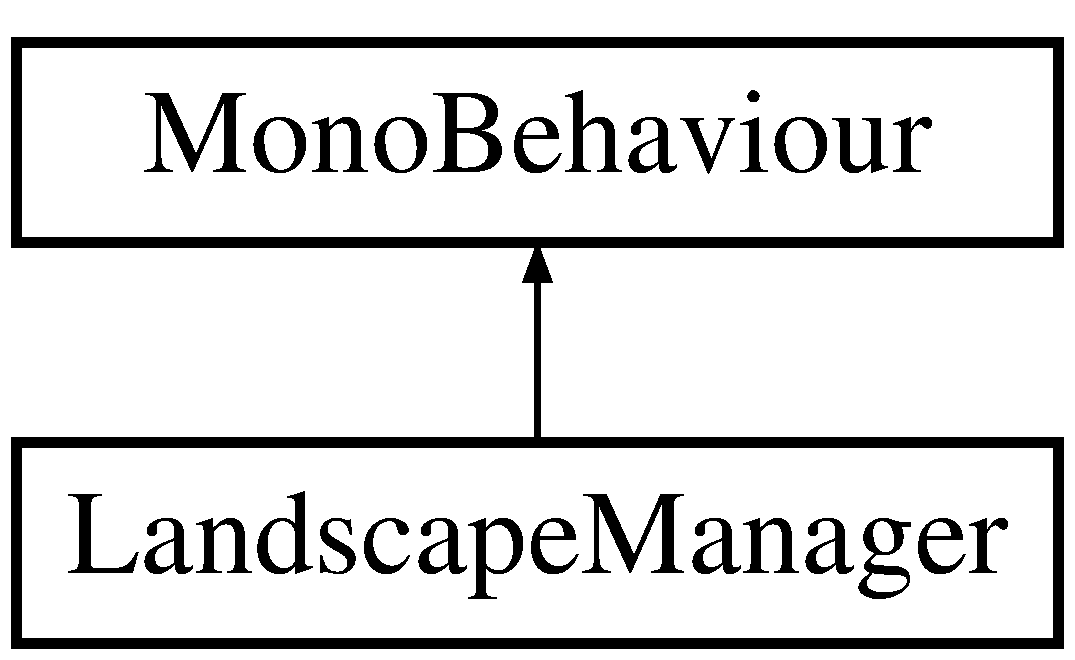
\includegraphics[height=2.000000cm]{class_landscape_manager}
\end{center}
\end{figure}
\subsection*{Private Member Functions}
\begin{DoxyCompactItemize}
\item 
void \hyperlink{class_landscape_manager_a5954eb34a23ac9f409c883b0a4bac033}{Start} ()
\item 
void \hyperlink{class_landscape_manager_afa615d6914c117affbe6b97e0b552502}{Update} ()
\end{DoxyCompactItemize}
\subsection*{Private Attributes}
\begin{DoxyCompactItemize}
\item 
\hyperlink{class_landscape_builder}{Landscape\+Builder} \hyperlink{class_landscape_manager_aa8cb7cbe6921ddb36a5aa73864556a56}{m\+\_\+landscape\+Builder}
\begin{DoxyCompactList}\small\item\em The builder class which \hyperlink{class_landscape_manager}{Landscape\+Manager} uses to get Landscapes. \end{DoxyCompactList}\end{DoxyCompactItemize}


\subsection{Member Function Documentation}
\mbox{\Hypertarget{class_landscape_manager_a5954eb34a23ac9f409c883b0a4bac033}\label{class_landscape_manager_a5954eb34a23ac9f409c883b0a4bac033}} 
\index{Landscape\+Manager@{Landscape\+Manager}!Start@{Start}}
\index{Start@{Start}!Landscape\+Manager@{Landscape\+Manager}}
\subsubsection{\texorpdfstring{Start()}{Start()}}
{\footnotesize\ttfamily void Landscape\+Manager.\+Start (\begin{DoxyParamCaption}{ }\end{DoxyParamCaption})\hspace{0.3cm}{\ttfamily [private]}}

\mbox{\Hypertarget{class_landscape_manager_afa615d6914c117affbe6b97e0b552502}\label{class_landscape_manager_afa615d6914c117affbe6b97e0b552502}} 
\index{Landscape\+Manager@{Landscape\+Manager}!Update@{Update}}
\index{Update@{Update}!Landscape\+Manager@{Landscape\+Manager}}
\subsubsection{\texorpdfstring{Update()}{Update()}}
{\footnotesize\ttfamily void Landscape\+Manager.\+Update (\begin{DoxyParamCaption}{ }\end{DoxyParamCaption})\hspace{0.3cm}{\ttfamily [private]}}



\subsection{Member Data Documentation}
\mbox{\Hypertarget{class_landscape_manager_aa8cb7cbe6921ddb36a5aa73864556a56}\label{class_landscape_manager_aa8cb7cbe6921ddb36a5aa73864556a56}} 
\index{Landscape\+Manager@{Landscape\+Manager}!m\+\_\+landscape\+Builder@{m\+\_\+landscape\+Builder}}
\index{m\+\_\+landscape\+Builder@{m\+\_\+landscape\+Builder}!Landscape\+Manager@{Landscape\+Manager}}
\subsubsection{\texorpdfstring{m\+\_\+landscape\+Builder}{m\_landscapeBuilder}}
{\footnotesize\ttfamily \hyperlink{class_landscape_builder}{Landscape\+Builder} Landscape\+Manager.\+m\+\_\+landscape\+Builder\hspace{0.3cm}{\ttfamily [private]}}



The builder class which \hyperlink{class_landscape_manager}{Landscape\+Manager} uses to get Landscapes. 



The documentation for this class was generated from the following file\+:\begin{DoxyCompactItemize}
\item 
Assets/\hyperlink{_landscape_manager_8cs}{Landscape\+Manager.\+cs}\end{DoxyCompactItemize}

\hypertarget{class_mountain}{}\section{Mountain Class Reference}
\label{class_mountain}\index{Mountain@{Mountain}}
Inheritance diagram for Mountain\+:\begin{figure}[H]
\begin{center}
\leavevmode
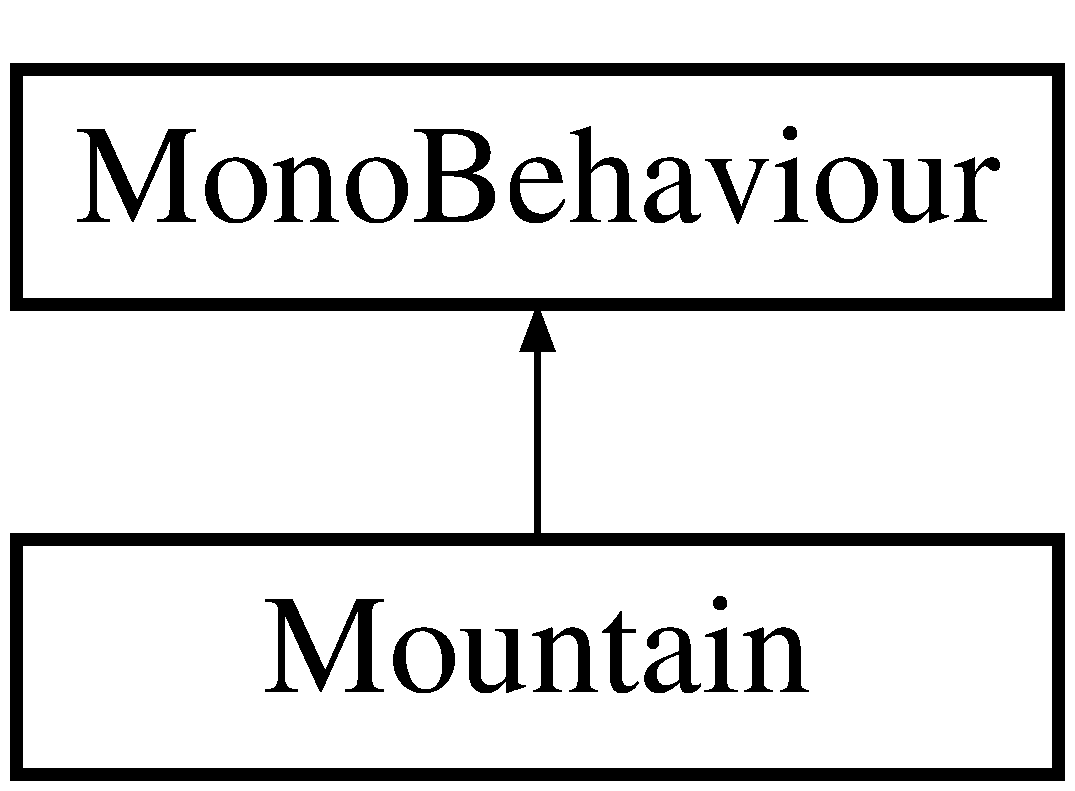
\includegraphics[height=2.000000cm]{class_mountain}
\end{center}
\end{figure}
\subsection*{Private Member Functions}
\begin{DoxyCompactItemize}
\item 
void \hyperlink{class_mountain_ad820629d33b788dc3a95dc92330ded8c}{Start} ()
\item 
void \hyperlink{class_mountain_a5083994b8a81bb115256ede2566fa8e9}{Update} ()
\end{DoxyCompactItemize}


\subsection{Member Function Documentation}
\mbox{\Hypertarget{class_mountain_ad820629d33b788dc3a95dc92330ded8c}\label{class_mountain_ad820629d33b788dc3a95dc92330ded8c}} 
\index{Mountain@{Mountain}!Start@{Start}}
\index{Start@{Start}!Mountain@{Mountain}}
\subsubsection{\texorpdfstring{Start()}{Start()}}
{\footnotesize\ttfamily void Mountain.\+Start (\begin{DoxyParamCaption}{ }\end{DoxyParamCaption})\hspace{0.3cm}{\ttfamily [private]}}

\mbox{\Hypertarget{class_mountain_a5083994b8a81bb115256ede2566fa8e9}\label{class_mountain_a5083994b8a81bb115256ede2566fa8e9}} 
\index{Mountain@{Mountain}!Update@{Update}}
\index{Update@{Update}!Mountain@{Mountain}}
\subsubsection{\texorpdfstring{Update()}{Update()}}
{\footnotesize\ttfamily void Mountain.\+Update (\begin{DoxyParamCaption}{ }\end{DoxyParamCaption})\hspace{0.3cm}{\ttfamily [private]}}



The documentation for this class was generated from the following file\+:\begin{DoxyCompactItemize}
\item 
Assets/\hyperlink{_mountain_8cs}{Mountain.\+cs}\end{DoxyCompactItemize}

\hypertarget{class_mouse_input}{}\section{Mouse\+Input Class Reference}
\label{class_mouse_input}\index{Mouse\+Input@{Mouse\+Input}}
Inheritance diagram for Mouse\+Input\+:\begin{figure}[H]
\begin{center}
\leavevmode
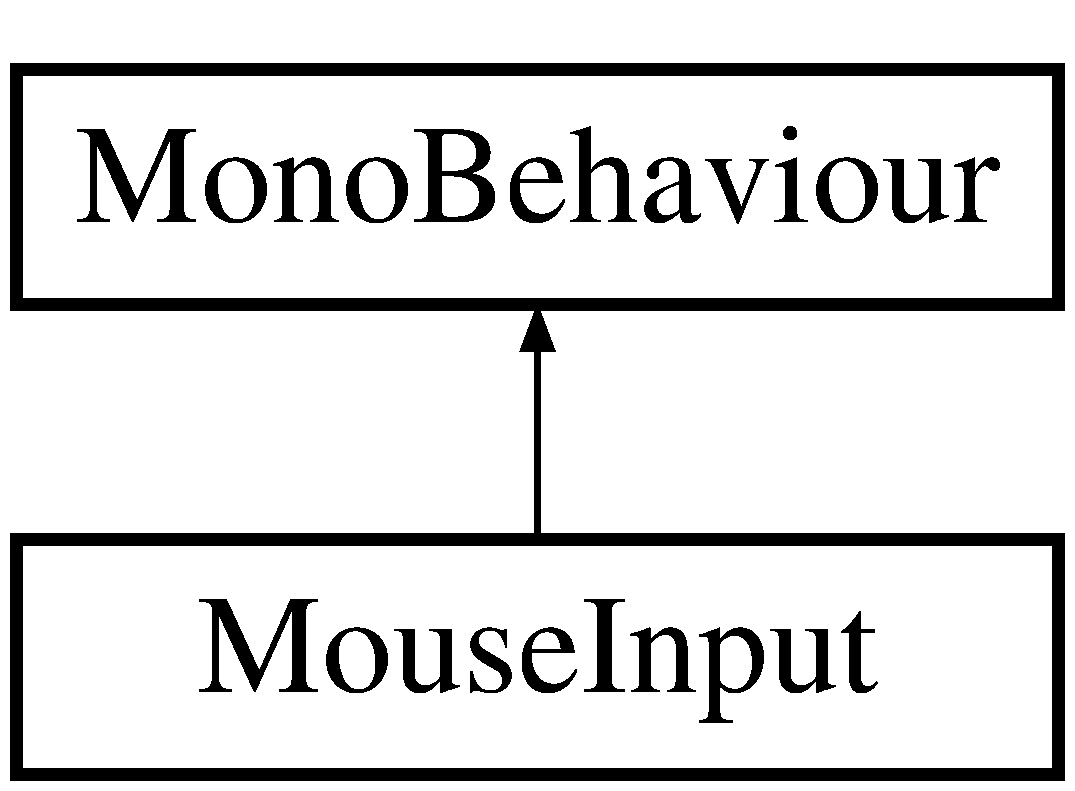
\includegraphics[height=2.000000cm]{class_mouse_input}
\end{center}
\end{figure}
\subsection*{Private Member Functions}
\begin{DoxyCompactItemize}
\item 
void \hyperlink{class_mouse_input_a3474cace48c31c81738e8473501bd8e9}{Start} ()
\item 
void \hyperlink{class_mouse_input_a54020c3263b04ebec5052eb540d815fe}{Update} ()
\end{DoxyCompactItemize}


\subsection{Member Function Documentation}
\mbox{\Hypertarget{class_mouse_input_a3474cace48c31c81738e8473501bd8e9}\label{class_mouse_input_a3474cace48c31c81738e8473501bd8e9}} 
\index{Mouse\+Input@{Mouse\+Input}!Start@{Start}}
\index{Start@{Start}!Mouse\+Input@{Mouse\+Input}}
\subsubsection{\texorpdfstring{Start()}{Start()}}
{\footnotesize\ttfamily void Mouse\+Input.\+Start (\begin{DoxyParamCaption}{ }\end{DoxyParamCaption})\hspace{0.3cm}{\ttfamily [private]}}

\mbox{\Hypertarget{class_mouse_input_a54020c3263b04ebec5052eb540d815fe}\label{class_mouse_input_a54020c3263b04ebec5052eb540d815fe}} 
\index{Mouse\+Input@{Mouse\+Input}!Update@{Update}}
\index{Update@{Update}!Mouse\+Input@{Mouse\+Input}}
\subsubsection{\texorpdfstring{Update()}{Update()}}
{\footnotesize\ttfamily void Mouse\+Input.\+Update (\begin{DoxyParamCaption}{ }\end{DoxyParamCaption})\hspace{0.3cm}{\ttfamily [private]}}



The documentation for this class was generated from the following file\+:\begin{DoxyCompactItemize}
\item 
Assets/\hyperlink{_mouse_input_8cs}{Mouse\+Input.\+cs}\end{DoxyCompactItemize}

\hypertarget{class_panel}{}\section{Panel Class Reference}
\label{class_panel}\index{Panel@{Panel}}
Inheritance diagram for Panel\+:\begin{figure}[H]
\begin{center}
\leavevmode
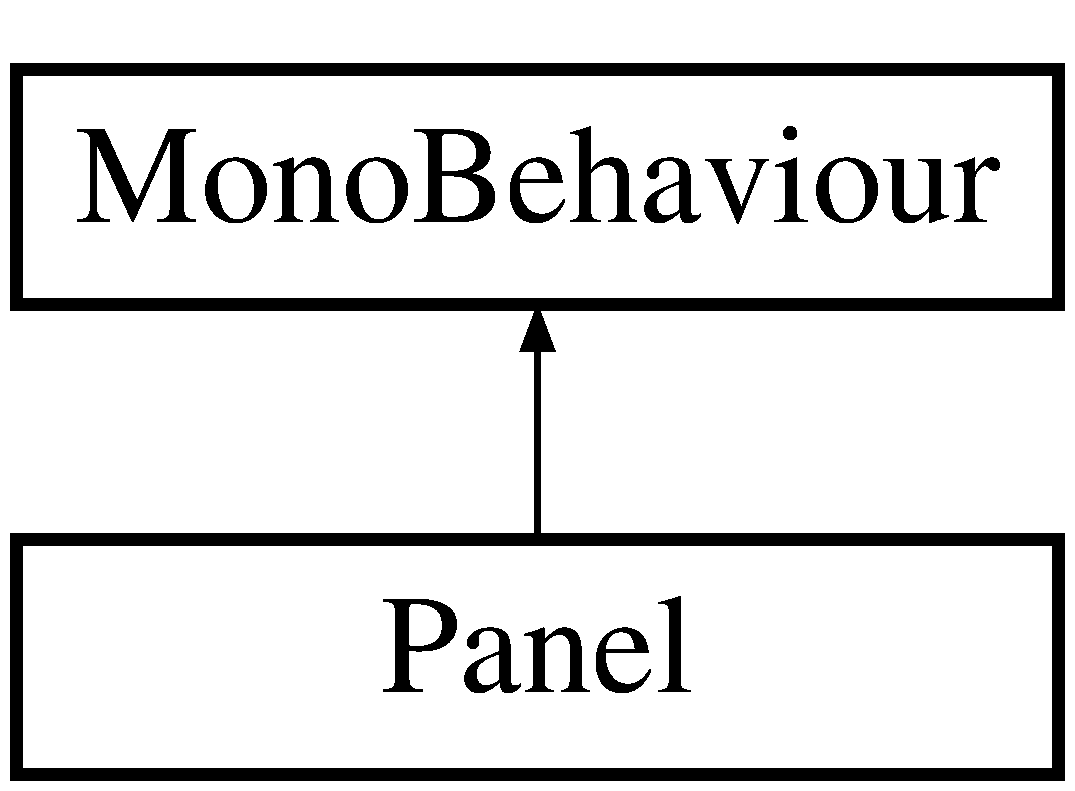
\includegraphics[height=2.000000cm]{class_panel}
\end{center}
\end{figure}
\subsection*{Private Member Functions}
\begin{DoxyCompactItemize}
\item 
void \hyperlink{class_panel_aa88b843bea8cee778539d808204ac362}{Start} ()
\item 
void \hyperlink{class_panel_ad9014f25d89f2d6219c9c0e27205edea}{Update} ()
\end{DoxyCompactItemize}


\subsection{Member Function Documentation}
\mbox{\Hypertarget{class_panel_aa88b843bea8cee778539d808204ac362}\label{class_panel_aa88b843bea8cee778539d808204ac362}} 
\index{Panel@{Panel}!Start@{Start}}
\index{Start@{Start}!Panel@{Panel}}
\subsubsection{\texorpdfstring{Start()}{Start()}}
{\footnotesize\ttfamily void Panel.\+Start (\begin{DoxyParamCaption}{ }\end{DoxyParamCaption})\hspace{0.3cm}{\ttfamily [private]}}

\mbox{\Hypertarget{class_panel_ad9014f25d89f2d6219c9c0e27205edea}\label{class_panel_ad9014f25d89f2d6219c9c0e27205edea}} 
\index{Panel@{Panel}!Update@{Update}}
\index{Update@{Update}!Panel@{Panel}}
\subsubsection{\texorpdfstring{Update()}{Update()}}
{\footnotesize\ttfamily void Panel.\+Update (\begin{DoxyParamCaption}{ }\end{DoxyParamCaption})\hspace{0.3cm}{\ttfamily [private]}}



The documentation for this class was generated from the following file\+:\begin{DoxyCompactItemize}
\item 
Assets/\hyperlink{_panel_8cs}{Panel.\+cs}\end{DoxyCompactItemize}

\hypertarget{class_plain}{}\section{Plain Class Reference}
\label{class_plain}\index{Plain@{Plain}}
Inheritance diagram for Plain\+:\begin{figure}[H]
\begin{center}
\leavevmode
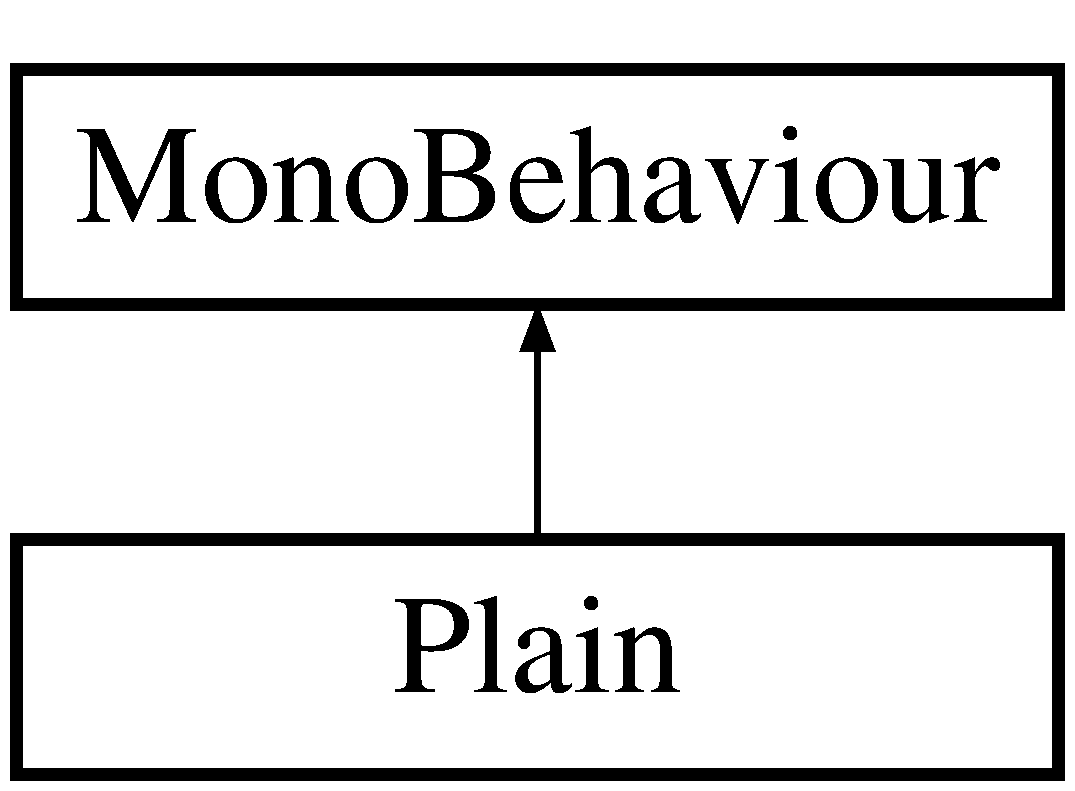
\includegraphics[height=2.000000cm]{class_plain}
\end{center}
\end{figure}
\subsection*{Private Member Functions}
\begin{DoxyCompactItemize}
\item 
void \hyperlink{class_plain_ac16b23286105687d19efee2664036817}{Start} ()
\item 
void \hyperlink{class_plain_aa6987996964007fcbaee1c9952d97a48}{Update} ()
\end{DoxyCompactItemize}


\subsection{Member Function Documentation}
\mbox{\Hypertarget{class_plain_ac16b23286105687d19efee2664036817}\label{class_plain_ac16b23286105687d19efee2664036817}} 
\index{Plain@{Plain}!Start@{Start}}
\index{Start@{Start}!Plain@{Plain}}
\subsubsection{\texorpdfstring{Start()}{Start()}}
{\footnotesize\ttfamily void Plain.\+Start (\begin{DoxyParamCaption}{ }\end{DoxyParamCaption})\hspace{0.3cm}{\ttfamily [private]}}

\mbox{\Hypertarget{class_plain_aa6987996964007fcbaee1c9952d97a48}\label{class_plain_aa6987996964007fcbaee1c9952d97a48}} 
\index{Plain@{Plain}!Update@{Update}}
\index{Update@{Update}!Plain@{Plain}}
\subsubsection{\texorpdfstring{Update()}{Update()}}
{\footnotesize\ttfamily void Plain.\+Update (\begin{DoxyParamCaption}{ }\end{DoxyParamCaption})\hspace{0.3cm}{\ttfamily [private]}}



The documentation for this class was generated from the following file\+:\begin{DoxyCompactItemize}
\item 
Assets/\hyperlink{_plain_8cs}{Plain.\+cs}\end{DoxyCompactItemize}

\hypertarget{class_river}{}\section{River Class Reference}
\label{class_river}\index{River@{River}}
Inheritance diagram for River\+:\begin{figure}[H]
\begin{center}
\leavevmode
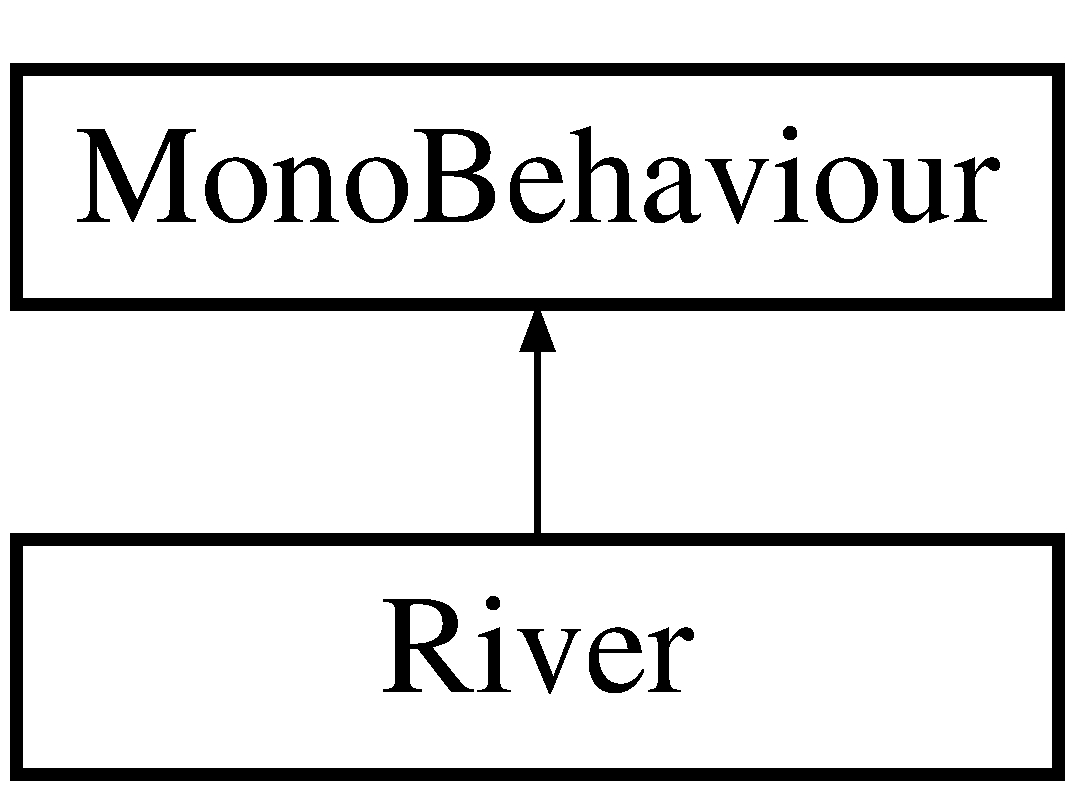
\includegraphics[height=2.000000cm]{class_river}
\end{center}
\end{figure}
\subsection*{Private Member Functions}
\begin{DoxyCompactItemize}
\item 
void \hyperlink{class_river_a993c5fb5b5ec86697e2b2416fd538b27}{Start} ()
\item 
void \hyperlink{class_river_ad320cf21a361e0223971150bf96dcaa6}{Update} ()
\end{DoxyCompactItemize}


\subsection{Member Function Documentation}
\mbox{\Hypertarget{class_river_a993c5fb5b5ec86697e2b2416fd538b27}\label{class_river_a993c5fb5b5ec86697e2b2416fd538b27}} 
\index{River@{River}!Start@{Start}}
\index{Start@{Start}!River@{River}}
\subsubsection{\texorpdfstring{Start()}{Start()}}
{\footnotesize\ttfamily void River.\+Start (\begin{DoxyParamCaption}{ }\end{DoxyParamCaption})\hspace{0.3cm}{\ttfamily [private]}}

\mbox{\Hypertarget{class_river_ad320cf21a361e0223971150bf96dcaa6}\label{class_river_ad320cf21a361e0223971150bf96dcaa6}} 
\index{River@{River}!Update@{Update}}
\index{Update@{Update}!River@{River}}
\subsubsection{\texorpdfstring{Update()}{Update()}}
{\footnotesize\ttfamily void River.\+Update (\begin{DoxyParamCaption}{ }\end{DoxyParamCaption})\hspace{0.3cm}{\ttfamily [private]}}



The documentation for this class was generated from the following file\+:\begin{DoxyCompactItemize}
\item 
Assets/\hyperlink{_river_8cs}{River.\+cs}\end{DoxyCompactItemize}

\hypertarget{class_scene_manager}{}\section{Scene\+Manager Class Reference}
\label{class_scene_manager}\index{Scene\+Manager@{Scene\+Manager}}
Inheritance diagram for Scene\+Manager\+:\begin{figure}[H]
\begin{center}
\leavevmode
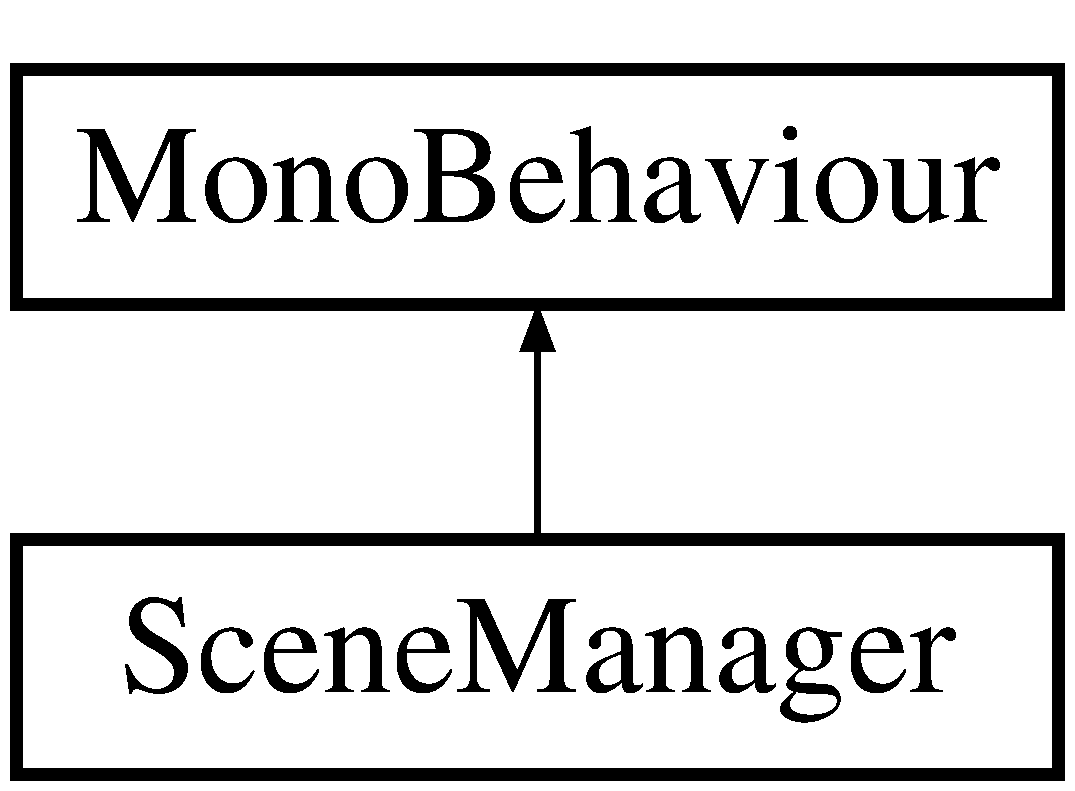
\includegraphics[height=2.000000cm]{class_scene_manager}
\end{center}
\end{figure}
\subsection*{Private Member Functions}
\begin{DoxyCompactItemize}
\item 
void \hyperlink{class_scene_manager_a86cc86842e457ed6c9d3268df97e1f9e}{Start} ()
\item 
void \hyperlink{class_scene_manager_a1700705e183249b1b8c6d95b8d044f69}{Update} ()
\end{DoxyCompactItemize}
\subsection*{Private Attributes}
\begin{DoxyCompactItemize}
\item 
\hyperlink{class_entity_manager}{Entity\+Manager} \hyperlink{class_scene_manager_abf81d312ff06974f7d47b03870e1578a}{m\+\_\+entity\+Manager}
\item 
\hyperlink{class_landscape_manager}{Landscape\+Manager} \hyperlink{class_scene_manager_a801b5db7fc9747ed992992b20d523e8a}{m\+\_\+landscape\+Manager}
\begin{DoxyCompactList}\small\item\em The manager class which \hyperlink{class_scene_manager}{Scene\+Manager} uses to get landscapes for the scene. \end{DoxyCompactList}\end{DoxyCompactItemize}


\subsection{Member Function Documentation}
\mbox{\Hypertarget{class_scene_manager_a86cc86842e457ed6c9d3268df97e1f9e}\label{class_scene_manager_a86cc86842e457ed6c9d3268df97e1f9e}} 
\index{Scene\+Manager@{Scene\+Manager}!Start@{Start}}
\index{Start@{Start}!Scene\+Manager@{Scene\+Manager}}
\subsubsection{\texorpdfstring{Start()}{Start()}}
{\footnotesize\ttfamily void Scene\+Manager.\+Start (\begin{DoxyParamCaption}{ }\end{DoxyParamCaption})\hspace{0.3cm}{\ttfamily [private]}}

\mbox{\Hypertarget{class_scene_manager_a1700705e183249b1b8c6d95b8d044f69}\label{class_scene_manager_a1700705e183249b1b8c6d95b8d044f69}} 
\index{Scene\+Manager@{Scene\+Manager}!Update@{Update}}
\index{Update@{Update}!Scene\+Manager@{Scene\+Manager}}
\subsubsection{\texorpdfstring{Update()}{Update()}}
{\footnotesize\ttfamily void Scene\+Manager.\+Update (\begin{DoxyParamCaption}{ }\end{DoxyParamCaption})\hspace{0.3cm}{\ttfamily [private]}}



\subsection{Member Data Documentation}
\mbox{\Hypertarget{class_scene_manager_abf81d312ff06974f7d47b03870e1578a}\label{class_scene_manager_abf81d312ff06974f7d47b03870e1578a}} 
\index{Scene\+Manager@{Scene\+Manager}!m\+\_\+entity\+Manager@{m\+\_\+entity\+Manager}}
\index{m\+\_\+entity\+Manager@{m\+\_\+entity\+Manager}!Scene\+Manager@{Scene\+Manager}}
\subsubsection{\texorpdfstring{m\+\_\+entity\+Manager}{m\_entityManager}}
{\footnotesize\ttfamily \hyperlink{class_entity_manager}{Entity\+Manager} Scene\+Manager.\+m\+\_\+entity\+Manager\hspace{0.3cm}{\ttfamily [private]}}

brief The manager class which \hyperlink{class_scene_manager}{Scene\+Manager} uses to get entities for the scene. \mbox{\Hypertarget{class_scene_manager_a801b5db7fc9747ed992992b20d523e8a}\label{class_scene_manager_a801b5db7fc9747ed992992b20d523e8a}} 
\index{Scene\+Manager@{Scene\+Manager}!m\+\_\+landscape\+Manager@{m\+\_\+landscape\+Manager}}
\index{m\+\_\+landscape\+Manager@{m\+\_\+landscape\+Manager}!Scene\+Manager@{Scene\+Manager}}
\subsubsection{\texorpdfstring{m\+\_\+landscape\+Manager}{m\_landscapeManager}}
{\footnotesize\ttfamily \hyperlink{class_landscape_manager}{Landscape\+Manager} Scene\+Manager.\+m\+\_\+landscape\+Manager\hspace{0.3cm}{\ttfamily [private]}}



The manager class which \hyperlink{class_scene_manager}{Scene\+Manager} uses to get landscapes for the scene. 



The documentation for this class was generated from the following file\+:\begin{DoxyCompactItemize}
\item 
Assets/\hyperlink{_scene_manager_8cs}{Scene\+Manager.\+cs}\end{DoxyCompactItemize}

\hypertarget{class_third_person_camera}{}\section{Third\+Person\+Camera Class Reference}
\label{class_third_person_camera}\index{Third\+Person\+Camera@{Third\+Person\+Camera}}
Inheritance diagram for Third\+Person\+Camera\+:\begin{figure}[H]
\begin{center}
\leavevmode
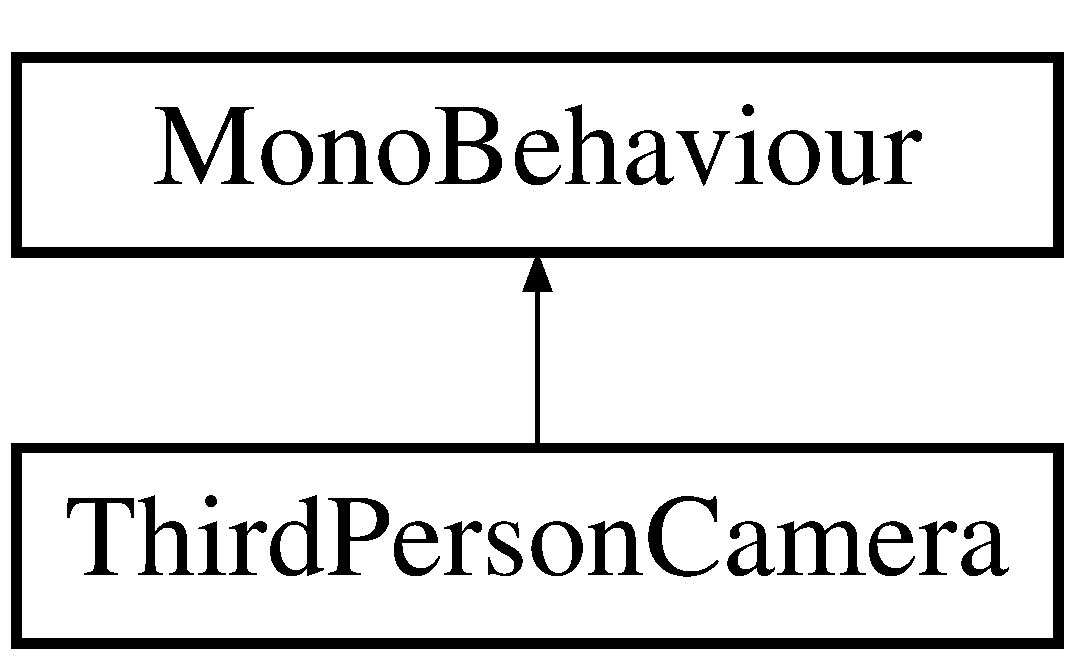
\includegraphics[height=2.000000cm]{class_third_person_camera}
\end{center}
\end{figure}
\subsection*{Private Member Functions}
\begin{DoxyCompactItemize}
\item 
void \hyperlink{class_third_person_camera_a2ef6a7e16a24068ef08990e18630c047}{Start} ()
\item 
void \hyperlink{class_third_person_camera_a20036aa1bbcabcff1f0c82d18300355d}{Update} ()
\end{DoxyCompactItemize}


\subsection{Member Function Documentation}
\mbox{\Hypertarget{class_third_person_camera_a2ef6a7e16a24068ef08990e18630c047}\label{class_third_person_camera_a2ef6a7e16a24068ef08990e18630c047}} 
\index{Third\+Person\+Camera@{Third\+Person\+Camera}!Start@{Start}}
\index{Start@{Start}!Third\+Person\+Camera@{Third\+Person\+Camera}}
\subsubsection{\texorpdfstring{Start()}{Start()}}
{\footnotesize\ttfamily void Third\+Person\+Camera.\+Start (\begin{DoxyParamCaption}{ }\end{DoxyParamCaption})\hspace{0.3cm}{\ttfamily [private]}}

\mbox{\Hypertarget{class_third_person_camera_a20036aa1bbcabcff1f0c82d18300355d}\label{class_third_person_camera_a20036aa1bbcabcff1f0c82d18300355d}} 
\index{Third\+Person\+Camera@{Third\+Person\+Camera}!Update@{Update}}
\index{Update@{Update}!Third\+Person\+Camera@{Third\+Person\+Camera}}
\subsubsection{\texorpdfstring{Update()}{Update()}}
{\footnotesize\ttfamily void Third\+Person\+Camera.\+Update (\begin{DoxyParamCaption}{ }\end{DoxyParamCaption})\hspace{0.3cm}{\ttfamily [private]}}



The documentation for this class was generated from the following file\+:\begin{DoxyCompactItemize}
\item 
Assets/\hyperlink{_third_person_camera_8cs}{Third\+Person\+Camera.\+cs}\end{DoxyCompactItemize}

\hypertarget{class_touch_input}{}\section{Touch\+Input Class Reference}
\label{class_touch_input}\index{Touch\+Input@{Touch\+Input}}
Inheritance diagram for Touch\+Input\+:\begin{figure}[H]
\begin{center}
\leavevmode
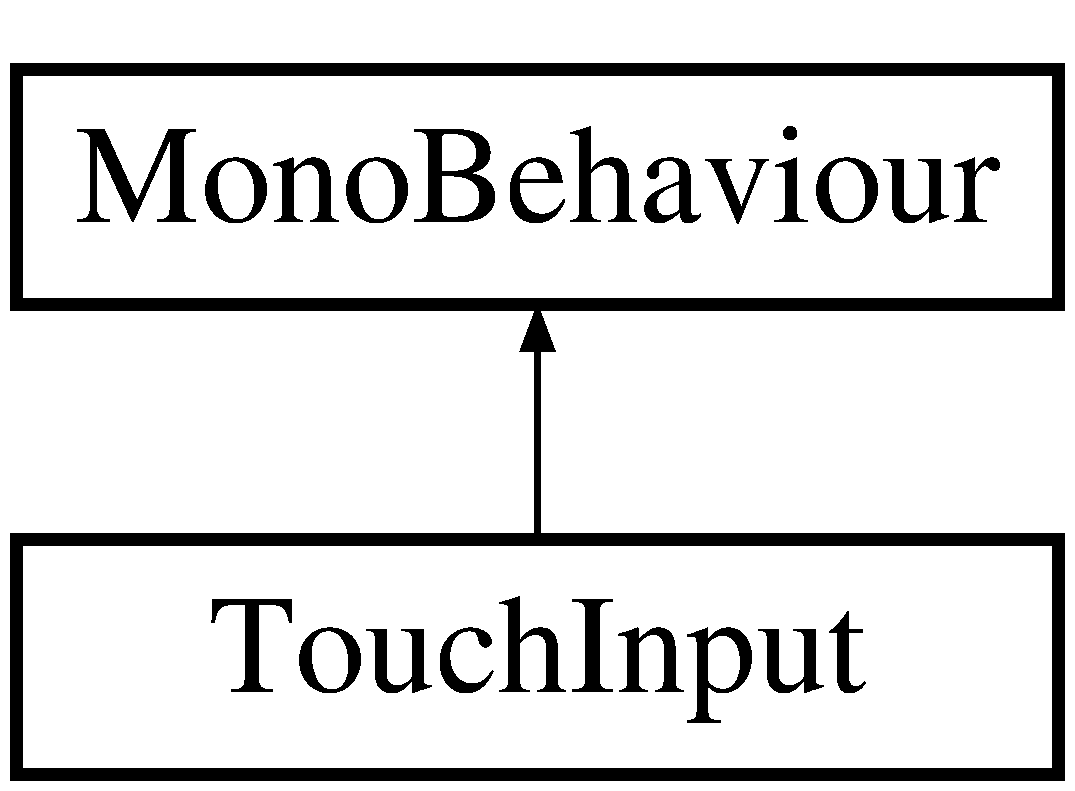
\includegraphics[height=2.000000cm]{class_touch_input}
\end{center}
\end{figure}
\subsection*{Private Member Functions}
\begin{DoxyCompactItemize}
\item 
void \hyperlink{class_touch_input_a66648591e7b990dff543e5dca46c5784}{Start} ()
\item 
void \hyperlink{class_touch_input_a5d0947600e2d12b72c8e76e67c9ceeca}{Update} ()
\end{DoxyCompactItemize}


\subsection{Member Function Documentation}
\mbox{\Hypertarget{class_touch_input_a66648591e7b990dff543e5dca46c5784}\label{class_touch_input_a66648591e7b990dff543e5dca46c5784}} 
\index{Touch\+Input@{Touch\+Input}!Start@{Start}}
\index{Start@{Start}!Touch\+Input@{Touch\+Input}}
\subsubsection{\texorpdfstring{Start()}{Start()}}
{\footnotesize\ttfamily void Touch\+Input.\+Start (\begin{DoxyParamCaption}{ }\end{DoxyParamCaption})\hspace{0.3cm}{\ttfamily [private]}}

\mbox{\Hypertarget{class_touch_input_a5d0947600e2d12b72c8e76e67c9ceeca}\label{class_touch_input_a5d0947600e2d12b72c8e76e67c9ceeca}} 
\index{Touch\+Input@{Touch\+Input}!Update@{Update}}
\index{Update@{Update}!Touch\+Input@{Touch\+Input}}
\subsubsection{\texorpdfstring{Update()}{Update()}}
{\footnotesize\ttfamily void Touch\+Input.\+Update (\begin{DoxyParamCaption}{ }\end{DoxyParamCaption})\hspace{0.3cm}{\ttfamily [private]}}



The documentation for this class was generated from the following file\+:\begin{DoxyCompactItemize}
\item 
Assets/\hyperlink{_touch_input_8cs}{Touch\+Input.\+cs}\end{DoxyCompactItemize}

\hypertarget{class_u_i_manager}{}\section{U\+I\+Manager Class Reference}
\label{class_u_i_manager}\index{U\+I\+Manager@{U\+I\+Manager}}
Inheritance diagram for U\+I\+Manager\+:\begin{figure}[H]
\begin{center}
\leavevmode
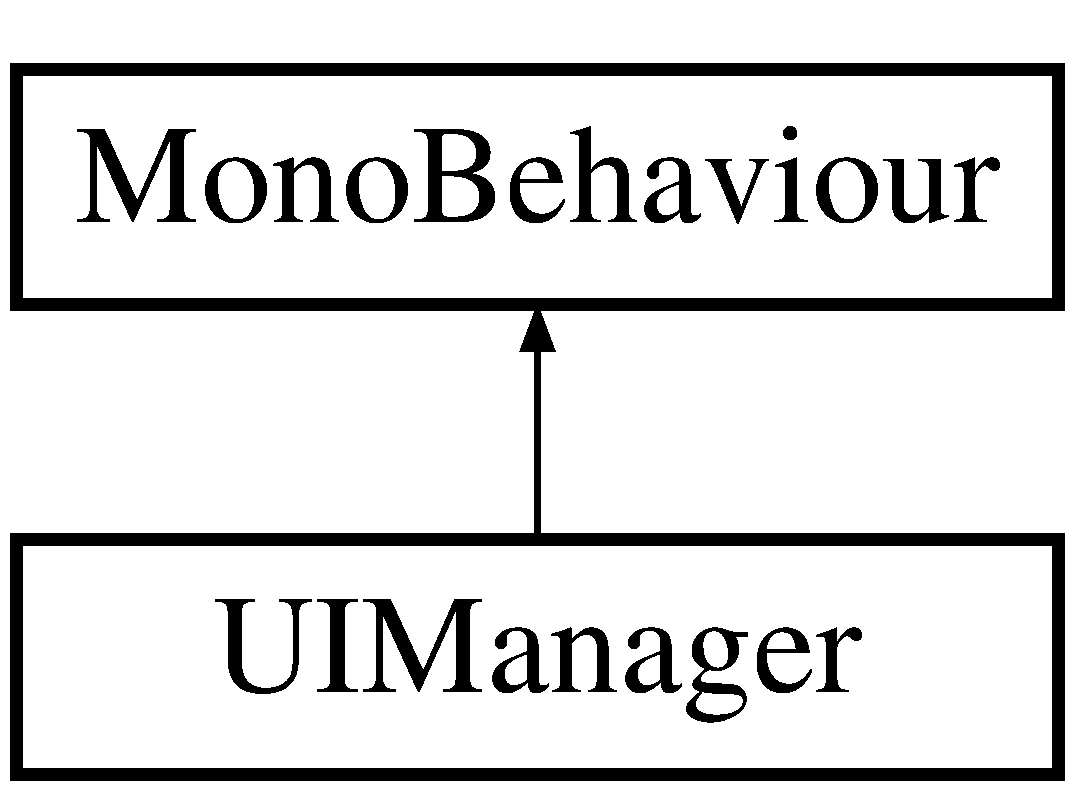
\includegraphics[height=2.000000cm]{class_u_i_manager}
\end{center}
\end{figure}
\subsection*{Private Member Functions}
\begin{DoxyCompactItemize}
\item 
void \hyperlink{class_u_i_manager_a2bd6b48b13b9e14e6292e4b713f59584}{Start} ()
\item 
void \hyperlink{class_u_i_manager_a6e2db9f2d98e70ccc4864d3af73f1b9e}{Update} ()
\end{DoxyCompactItemize}


\subsection{Member Function Documentation}
\mbox{\Hypertarget{class_u_i_manager_a2bd6b48b13b9e14e6292e4b713f59584}\label{class_u_i_manager_a2bd6b48b13b9e14e6292e4b713f59584}} 
\index{U\+I\+Manager@{U\+I\+Manager}!Start@{Start}}
\index{Start@{Start}!U\+I\+Manager@{U\+I\+Manager}}
\subsubsection{\texorpdfstring{Start()}{Start()}}
{\footnotesize\ttfamily void U\+I\+Manager.\+Start (\begin{DoxyParamCaption}{ }\end{DoxyParamCaption})\hspace{0.3cm}{\ttfamily [private]}}

\mbox{\Hypertarget{class_u_i_manager_a6e2db9f2d98e70ccc4864d3af73f1b9e}\label{class_u_i_manager_a6e2db9f2d98e70ccc4864d3af73f1b9e}} 
\index{U\+I\+Manager@{U\+I\+Manager}!Update@{Update}}
\index{Update@{Update}!U\+I\+Manager@{U\+I\+Manager}}
\subsubsection{\texorpdfstring{Update()}{Update()}}
{\footnotesize\ttfamily void U\+I\+Manager.\+Update (\begin{DoxyParamCaption}{ }\end{DoxyParamCaption})\hspace{0.3cm}{\ttfamily [private]}}



The documentation for this class was generated from the following file\+:\begin{DoxyCompactItemize}
\item 
Assets/\hyperlink{_u_i_manager_8cs}{U\+I\+Manager.\+cs}\end{DoxyCompactItemize}

\chapter{File Documentation}
\hypertarget{_animal_8cs}{}\section{Assets/\+Animal.cs File Reference}
\label{_animal_8cs}\index{Assets/\+Animal.\+cs@{Assets/\+Animal.\+cs}}
\subsection*{Classes}
\begin{DoxyCompactItemize}
\item 
class \hyperlink{class_animal}{Animal}
\end{DoxyCompactItemize}

\hypertarget{_button_8cs}{}\section{Assets/\+Button.cs File Reference}
\label{_button_8cs}\index{Assets/\+Button.\+cs@{Assets/\+Button.\+cs}}
\subsection*{Classes}
\begin{DoxyCompactItemize}
\item 
class \hyperlink{class_button}{Button}
\end{DoxyCompactItemize}

\hypertarget{_camera_manager_8cs}{}\section{Assets/\+Camera\+Manager.cs File Reference}
\label{_camera_manager_8cs}\index{Assets/\+Camera\+Manager.\+cs@{Assets/\+Camera\+Manager.\+cs}}
\subsection*{Classes}
\begin{DoxyCompactItemize}
\item 
class \hyperlink{class_camera_manager}{Camera\+Manager}
\end{DoxyCompactItemize}

\hypertarget{_cinematic_camera_8cs}{}\section{Assets/\+Cinematic\+Camera.cs File Reference}
\label{_cinematic_camera_8cs}\index{Assets/\+Cinematic\+Camera.\+cs@{Assets/\+Cinematic\+Camera.\+cs}}
\subsection*{Classes}
\begin{DoxyCompactItemize}
\item 
class \hyperlink{class_cinematic_camera}{Cinematic\+Camera}
\end{DoxyCompactItemize}

\hypertarget{_controller_input_8cs}{}\section{Assets/\+Controller\+Input.cs File Reference}
\label{_controller_input_8cs}\index{Assets/\+Controller\+Input.\+cs@{Assets/\+Controller\+Input.\+cs}}
\subsection*{Classes}
\begin{DoxyCompactItemize}
\item 
class \hyperlink{class_controller_input}{Controller\+Input}
\end{DoxyCompactItemize}

\hypertarget{_entity_8cs}{}\section{Assets/\+Entity.cs File Reference}
\label{_entity_8cs}\index{Assets/\+Entity.\+cs@{Assets/\+Entity.\+cs}}
\subsection*{Classes}
\begin{DoxyCompactItemize}
\item 
class \hyperlink{class_entity}{Entity}
\end{DoxyCompactItemize}

\hypertarget{_entity_builder_8cs}{}\section{Assets/\+Entity\+Builder.cs File Reference}
\label{_entity_builder_8cs}\index{Assets/\+Entity\+Builder.\+cs@{Assets/\+Entity\+Builder.\+cs}}
\subsection*{Classes}
\begin{DoxyCompactItemize}
\item 
class \hyperlink{class_entity_builder}{Entity\+Builder}
\end{DoxyCompactItemize}

\hypertarget{_entity_dictionary_8cs}{}\section{Assets/\+Entity\+Dictionary.cs File Reference}
\label{_entity_dictionary_8cs}\index{Assets/\+Entity\+Dictionary.\+cs@{Assets/\+Entity\+Dictionary.\+cs}}
\subsection*{Classes}
\begin{DoxyCompactItemize}
\item 
class \hyperlink{class_entity_dictionary}{Entity\+Dictionary}
\end{DoxyCompactItemize}

\hypertarget{_entity_manager_8cs}{}\section{Assets/\+Entity\+Manager.cs File Reference}
\label{_entity_manager_8cs}\index{Assets/\+Entity\+Manager.\+cs@{Assets/\+Entity\+Manager.\+cs}}
\subsection*{Classes}
\begin{DoxyCompactItemize}
\item 
class \hyperlink{class_entity_manager}{Entity\+Manager}
\end{DoxyCompactItemize}

\hypertarget{_enumerations_8cs}{}\section{Assets/\+Enumerations.cs File Reference}
\label{_enumerations_8cs}\index{Assets/\+Enumerations.\+cs@{Assets/\+Enumerations.\+cs}}
\subsection*{Classes}
\begin{DoxyCompactItemize}
\item 
class \hyperlink{class_enumerations}{Enumerations}
\end{DoxyCompactItemize}

\hypertarget{_first_person_camera_8cs}{}\section{Assets/\+First\+Person\+Camera.cs File Reference}
\label{_first_person_camera_8cs}\index{Assets/\+First\+Person\+Camera.\+cs@{Assets/\+First\+Person\+Camera.\+cs}}
\subsection*{Classes}
\begin{DoxyCompactItemize}
\item 
class \hyperlink{class_first_person_camera}{First\+Person\+Camera}
\end{DoxyCompactItemize}

\hypertarget{_forest_8cs}{}\section{Assets/\+Forest.cs File Reference}
\label{_forest_8cs}\index{Assets/\+Forest.\+cs@{Assets/\+Forest.\+cs}}
\subsection*{Classes}
\begin{DoxyCompactItemize}
\item 
class \hyperlink{class_forest}{Forest}
\end{DoxyCompactItemize}

\hypertarget{_graphic_8cs}{}\section{Assets/\+Graphic.cs File Reference}
\label{_graphic_8cs}\index{Assets/\+Graphic.\+cs@{Assets/\+Graphic.\+cs}}
\subsection*{Classes}
\begin{DoxyCompactItemize}
\item 
class \hyperlink{class_graphic}{Graphic}
\end{DoxyCompactItemize}

\hypertarget{_house_8cs}{}\section{Assets/\+House.cs File Reference}
\label{_house_8cs}\index{Assets/\+House.\+cs@{Assets/\+House.\+cs}}
\subsection*{Classes}
\begin{DoxyCompactItemize}
\item 
class \hyperlink{class_house}{House}
\end{DoxyCompactItemize}

\hypertarget{_human_8cs}{}\section{Assets/\+Human.cs File Reference}
\label{_human_8cs}\index{Assets/\+Human.\+cs@{Assets/\+Human.\+cs}}
\subsection*{Classes}
\begin{DoxyCompactItemize}
\item 
class \hyperlink{class_human}{Human}
\end{DoxyCompactItemize}

\hypertarget{_input_manager_8cs}{}\section{Assets/\+Input\+Manager.cs File Reference}
\label{_input_manager_8cs}\index{Assets/\+Input\+Manager.\+cs@{Assets/\+Input\+Manager.\+cs}}
\subsection*{Classes}
\begin{DoxyCompactItemize}
\item 
class \hyperlink{class_input_manager}{Input\+Manager}
\end{DoxyCompactItemize}

\hypertarget{_isometric_camera_8cs}{}\section{Assets/\+Isometric\+Camera.cs File Reference}
\label{_isometric_camera_8cs}\index{Assets/\+Isometric\+Camera.\+cs@{Assets/\+Isometric\+Camera.\+cs}}
\subsection*{Classes}
\begin{DoxyCompactItemize}
\item 
class \hyperlink{class_isometric_camera}{Isometric\+Camera}
\end{DoxyCompactItemize}

\hypertarget{_landscape_8cs}{}\section{Assets/\+Landscape.cs File Reference}
\label{_landscape_8cs}\index{Assets/\+Landscape.\+cs@{Assets/\+Landscape.\+cs}}
\subsection*{Classes}
\begin{DoxyCompactItemize}
\item 
class \hyperlink{class_landscape}{Landscape}
\end{DoxyCompactItemize}

\hypertarget{_landscape_builder_8cs}{}\section{Assets/\+Landscape\+Builder.cs File Reference}
\label{_landscape_builder_8cs}\index{Assets/\+Landscape\+Builder.\+cs@{Assets/\+Landscape\+Builder.\+cs}}
\subsection*{Classes}
\begin{DoxyCompactItemize}
\item 
class \hyperlink{class_landscape_builder}{Landscape\+Builder}
\end{DoxyCompactItemize}

\hypertarget{_landscape_dictionary_8cs}{}\section{Assets/\+Landscape\+Dictionary.cs File Reference}
\label{_landscape_dictionary_8cs}\index{Assets/\+Landscape\+Dictionary.\+cs@{Assets/\+Landscape\+Dictionary.\+cs}}
\subsection*{Classes}
\begin{DoxyCompactItemize}
\item 
class \hyperlink{class_landscape_dictionary}{Landscape\+Dictionary}
\end{DoxyCompactItemize}

\hypertarget{_landscape_manager_8cs}{}\section{Assets/\+Landscape\+Manager.cs File Reference}
\label{_landscape_manager_8cs}\index{Assets/\+Landscape\+Manager.\+cs@{Assets/\+Landscape\+Manager.\+cs}}
\subsection*{Classes}
\begin{DoxyCompactItemize}
\item 
class \hyperlink{class_landscape_manager}{Landscape\+Manager}
\end{DoxyCompactItemize}

\hypertarget{_mountain_8cs}{}\section{Assets/\+Mountain.cs File Reference}
\label{_mountain_8cs}\index{Assets/\+Mountain.\+cs@{Assets/\+Mountain.\+cs}}
\subsection*{Classes}
\begin{DoxyCompactItemize}
\item 
class \hyperlink{class_mountain}{Mountain}
\end{DoxyCompactItemize}

\hypertarget{_mouse_input_8cs}{}\section{Assets/\+Mouse\+Input.cs File Reference}
\label{_mouse_input_8cs}\index{Assets/\+Mouse\+Input.\+cs@{Assets/\+Mouse\+Input.\+cs}}
\subsection*{Classes}
\begin{DoxyCompactItemize}
\item 
class \hyperlink{class_mouse_input}{Mouse\+Input}
\end{DoxyCompactItemize}

\hypertarget{_panel_8cs}{}\section{Assets/\+Panel.cs File Reference}
\label{_panel_8cs}\index{Assets/\+Panel.\+cs@{Assets/\+Panel.\+cs}}
\subsection*{Classes}
\begin{DoxyCompactItemize}
\item 
class \hyperlink{class_panel}{Panel}
\end{DoxyCompactItemize}

\hypertarget{_plain_8cs}{}\section{Assets/\+Plain.cs File Reference}
\label{_plain_8cs}\index{Assets/\+Plain.\+cs@{Assets/\+Plain.\+cs}}
\subsection*{Classes}
\begin{DoxyCompactItemize}
\item 
class \hyperlink{class_plain}{Plain}
\end{DoxyCompactItemize}

\hypertarget{_river_8cs}{}\section{Assets/\+River.cs File Reference}
\label{_river_8cs}\index{Assets/\+River.\+cs@{Assets/\+River.\+cs}}
\subsection*{Classes}
\begin{DoxyCompactItemize}
\item 
class \hyperlink{class_river}{River}
\end{DoxyCompactItemize}

\hypertarget{_scene_manager_8cs}{}\section{Assets/\+Scene\+Manager.cs File Reference}
\label{_scene_manager_8cs}\index{Assets/\+Scene\+Manager.\+cs@{Assets/\+Scene\+Manager.\+cs}}
\subsection*{Classes}
\begin{DoxyCompactItemize}
\item 
class \hyperlink{class_scene_manager}{Scene\+Manager}
\end{DoxyCompactItemize}

\hypertarget{_third_person_camera_8cs}{}\section{Assets/\+Third\+Person\+Camera.cs File Reference}
\label{_third_person_camera_8cs}\index{Assets/\+Third\+Person\+Camera.\+cs@{Assets/\+Third\+Person\+Camera.\+cs}}
\subsection*{Classes}
\begin{DoxyCompactItemize}
\item 
class \hyperlink{class_third_person_camera}{Third\+Person\+Camera}
\end{DoxyCompactItemize}

\hypertarget{_touch_input_8cs}{}\section{Assets/\+Touch\+Input.cs File Reference}
\label{_touch_input_8cs}\index{Assets/\+Touch\+Input.\+cs@{Assets/\+Touch\+Input.\+cs}}
\subsection*{Classes}
\begin{DoxyCompactItemize}
\item 
class \hyperlink{class_touch_input}{Touch\+Input}
\end{DoxyCompactItemize}

\hypertarget{_u_i_manager_8cs}{}\section{Assets/\+U\+I\+Manager.cs File Reference}
\label{_u_i_manager_8cs}\index{Assets/\+U\+I\+Manager.\+cs@{Assets/\+U\+I\+Manager.\+cs}}
\subsection*{Classes}
\begin{DoxyCompactItemize}
\item 
class \hyperlink{class_u_i_manager}{U\+I\+Manager}
\end{DoxyCompactItemize}

\hypertarget{_r_e_a_d_m_e_8md}{}\section{R\+E\+A\+D\+M\+E.\+md File Reference}
\label{_r_e_a_d_m_e_8md}\index{R\+E\+A\+D\+M\+E.\+md@{R\+E\+A\+D\+M\+E.\+md}}

%--- End generated contents ---

% Index
\backmatter
\newpage
\phantomsection
\clearemptydoublepage
\addcontentsline{toc}{chapter}{Index}
\printindex

\end{document}
